\begin{questions}
    \ifnum \Set=1
        \ifnum \Version=1
\question[2] Determine the values of $r$ so that the differential equation $\displaystyle t^2y'' -4ty' +6y =0$ will have solutions of the form $\displaystyle y = t^r$ for $t>0$. Please show your work.
\ifnum \Solutions=1 {\color{DarkGreen} \\[12pt] 
\textbf{Solutions:} substitute $y=t^r$ into the equation to obtain:
\begin{align}
    0 &= t^2y'' -4ty' +6y \\
    &= t^2(t^r)'' - 4t(t^r)' + 6(t^r) \\ 
    &= t^2r(r-1)(t^{r-2}) - 4tr(t^{r-1}) + 6(t^r) \\ 
    &= r(r-1)(t^{r}) - 4r(t^{r}) + 6(t^r) \\ 
    &= r(r-1) - 4r + 6 \\ 
    &= r^2 - 5r + 6 \\ 
    &= (r-2)(r-3) 
\end{align}
Therefore $r=2,3$. 
} 
\else 
\fi\fi 

\ifnum \Version=6
\SecondOrderConstCo{5}{6}
\fi


\ifnum \Version=7
\SecondOrderCauchyEuler{2}{1}
\fi

\ifnum \Version=8
\SecondOrderConstCo{4}{8}
\fi


\ifnum \Version=9
\SecondOrderCauchyEuler{1}{3}
\fi


        \ifnum \Version=1

\question[2] A spring is hung from a horizontal surface as in the figure below. A mass of $m=0.2$ kg stretches the spring 0.04 m. Frictional forces also exert a force on the mass while it is moving that is proportional to the velocity of the mass. The proportionality constant for these frictional forces is 2 N s/m. The mass is then pulled down an additional 0.03 m and then released from rest. Assume that position of the mass, $y$, increases as the mass moves down. Write down an IVP based on this physical description that describes the position of the mass $y(t)$, as a function of time, $t$. You do not need to solve your IVP. \\[4pt]
\input{2023Summer/Quiz4/DiagramSpringMass}
\vspace{2cm}
\fi 


\ifnum \Version=2
\question[2] A small car with mass $m = 0.2$ kg is moving along a straight line on a horizontal surface. The car is attached to a spring. The spring exerts a force of $4$ N when it is extended a distance of $0.8$ meters from its equilibrium position. Frictional forces also exert a force on the car while it is moving that is proportional to the velocity of the car. The proportionality constant for these frictional forces is $0.6$ N s/m. The car also has an engine that pushes the car forward with a force of $F = 0.5t$ N. The car is released from rest after it is moved 0.01 m to the right of its equilibrium position. Assume that position of the car, $y$, increases as the car move to the right. Write down the IVP based on this physical description that describes the position of the car as a function of time, $t$. You do not need to solve your IVP. \\
\hspace{1cm}\begin{tikzpicture}
\tikzstyle{spring}=[thick,decorate,decoration={zigzag,pre length=0.3cm,post length=0.3cm,segment length=6}]
\tikzstyle{damper}=[thick,decoration={markings,  
  mark connection node=dmp,
  mark=at position 0.5 with 
  {
    \node (dmp) [thick,inner sep=0pt,transform shape,rotate=-90,minimum width=15pt,minimum height=3pt,draw=none] {};
    \draw [thick] ($(dmp.north east)+(2pt,0)$) -- (dmp.south east) -- (dmp.south west) -- ($(dmp.north west)+(2pt,0)$);
    \draw [thick] ($(dmp.north)+(0,-5pt)$) -- ($(dmp.north)+(0,5pt)$);
  }
}, decorate]

% WALL PATTERN
\tikzstyle{ground}=[fill,pattern=north east lines,draw=none,minimum width=0.5cm,minimum height=0.3cm,inner sep=0pt,outer sep=0pt]

% CART
\node [style={draw,outer sep=0pt,very thick}] (M) [minimum width=1cm, minimum height=1.0cm] {$m$};
% WHEELS
\draw [very thick] (M.south west) ++ (0.2cm,-0.125cm) circle (0.125cm)  (M.south east) ++ (-0.2cm,-0.125cm) circle (0.125cm);

% BOTTOM GROUND
\node (ground) [ground,anchor=north,yshift=-0.25cm,minimum width=5.6cm,xshift=-0.03cm] at (M.south) {};
\draw (ground.north east) -- (ground.north west);
\draw (ground.south east) -- (ground.south west);
\draw (ground.north east) -- (ground.south east);

% WEST WALL
\node (wall) [ground, rotate=-90, minimum width=3cm,xshift=-0.42cm,yshift=-3cm] {};
\draw (wall.north east) -- (wall.north west);
\draw (wall.north west) -- (wall.south west);
\draw (wall.south west) -- (wall.south east);
\draw (wall.south east) -- (wall.north east);

% DAMPER AND SPRING
\draw [spring] (wall.20) -- ($(M.north west)!(wall.20)!(M.south west)$);
% \node (y) at (wall.130) [yshift = 0.02cm,xshift=1.2cm] {$k$};

\end{tikzpicture}

\fi 

\ifnum \Version=3
\question[2] A small car with mass $m = 0.1$ kg is moving along a straight line on a horizontal surface. The car is attached to a spring. The spring exerts a force of $2$ N when it is extended a distance of $0.1$ meters from its equilibrium position. Frictional forces also exert a force on the car while it is moving that is proportional to the velocity of the car. The proportionality constant for these frictional forces is $0.3$ N s/m. The car also has an engine that pushes the car forward with a force of $F = 0.1$ N. The car is released from rest after it is moved 0.01 m to the left of its equilibrium position. Assume that position of the car, $y$, increases as the car move to the right. Write down the IVP based on this physical description that describes the position of the car as a function of time, $t$. You do not need to solve your IVP. \\
\hspace{1cm}\begin{tikzpicture}
\tikzstyle{spring}=[thick,decorate,decoration={zigzag,pre length=0.3cm,post length=0.3cm,segment length=6}]
\tikzstyle{damper}=[thick,decoration={markings,  
  mark connection node=dmp,
  mark=at position 0.5 with 
  {
    \node (dmp) [thick,inner sep=0pt,transform shape,rotate=-90,minimum width=15pt,minimum height=3pt,draw=none] {};
    \draw [thick] ($(dmp.north east)+(2pt,0)$) -- (dmp.south east) -- (dmp.south west) -- ($(dmp.north west)+(2pt,0)$);
    \draw [thick] ($(dmp.north)+(0,-5pt)$) -- ($(dmp.north)+(0,5pt)$);
  }
}, decorate]

% WALL PATTERN
\tikzstyle{ground}=[fill,pattern=north east lines,draw=none,minimum width=0.5cm,minimum height=0.3cm,inner sep=0pt,outer sep=0pt]

% CART
\node [style={draw,outer sep=0pt,very thick}] (M) [minimum width=1cm, minimum height=1.0cm] {$m$};
% WHEELS
\draw [very thick] (M.south west) ++ (0.2cm,-0.125cm) circle (0.125cm)  (M.south east) ++ (-0.2cm,-0.125cm) circle (0.125cm);

% BOTTOM GROUND
\node (ground) [ground,anchor=north,yshift=-0.25cm,minimum width=5.6cm,xshift=-0.03cm] at (M.south) {};
\draw (ground.north east) -- (ground.north west);
\draw (ground.south east) -- (ground.south west);
\draw (ground.north east) -- (ground.south east);

% WEST WALL
\node (wall) [ground, rotate=-90, minimum width=3cm,xshift=-0.42cm,yshift=-3cm] {};
\draw (wall.north east) -- (wall.north west);
\draw (wall.north west) -- (wall.south west);
\draw (wall.south west) -- (wall.south east);
\draw (wall.south east) -- (wall.north east);

% DAMPER AND SPRING
\draw [spring] (wall.20) -- ($(M.north west)!(wall.20)!(M.south west)$);
% \node (y) at (wall.130) [yshift = 0.02cm,xshift=1.2cm] {$k$};

\end{tikzpicture}

\fi 

\ifnum \Version=4
\question[2] A small car with mass $m = 0.2$ kg is moving along a straight line on a horizontal surface. The car is attached to a spring. The spring exerts a force of $4$ N when it is extended a distance of $0.8$ meters from its equilibrium position. Frictional forces also exert a force on the car while it is moving that is proportional to the velocity of the car. The proportionality constant for these frictional forces is $0.6$ N s/m. The car also has an engine that pushes the car forward with a force of $F = 0.5t$ N. The car is released from rest after it is moved 0.05 m to the left of its equilibrium position. Assume that position of the car, $y$, increases as the car move to the right. Write down the IVP based on this physical description that describes the position of the car as a function of time, $t$. You do not need to solve your IVP. \\
\hspace{1cm}\begin{tikzpicture}
\tikzstyle{spring}=[thick,decorate,decoration={zigzag,pre length=0.3cm,post length=0.3cm,segment length=6}]
\tikzstyle{damper}=[thick,decoration={markings,  
  mark connection node=dmp,
  mark=at position 0.5 with 
  {
    \node (dmp) [thick,inner sep=0pt,transform shape,rotate=-90,minimum width=15pt,minimum height=3pt,draw=none] {};
    \draw [thick] ($(dmp.north east)+(2pt,0)$) -- (dmp.south east) -- (dmp.south west) -- ($(dmp.north west)+(2pt,0)$);
    \draw [thick] ($(dmp.north)+(0,-5pt)$) -- ($(dmp.north)+(0,5pt)$);
  }
}, decorate]

% WALL PATTERN
\tikzstyle{ground}=[fill,pattern=north east lines,draw=none,minimum width=0.5cm,minimum height=0.3cm,inner sep=0pt,outer sep=0pt]

% CART
\node [style={draw,outer sep=0pt,very thick}] (M) [minimum width=1cm, minimum height=1.0cm] {$m$};
% WHEELS
\draw [very thick] (M.south west) ++ (0.2cm,-0.125cm) circle (0.125cm)  (M.south east) ++ (-0.2cm,-0.125cm) circle (0.125cm);

% BOTTOM GROUND
\node (ground) [ground,anchor=north,yshift=-0.25cm,minimum width=5.6cm,xshift=-0.03cm] at (M.south) {};
\draw (ground.north east) -- (ground.north west);
\draw (ground.south east) -- (ground.south west);
\draw (ground.north east) -- (ground.south east);

% WEST WALL
\node (wall) [ground, rotate=-90, minimum width=3cm,xshift=-0.42cm,yshift=-3cm] {};
\draw (wall.north east) -- (wall.north west);
\draw (wall.north west) -- (wall.south west);
\draw (wall.south west) -- (wall.south east);
\draw (wall.south east) -- (wall.north east);

% DAMPER AND SPRING
\draw [spring] (wall.20) -- ($(M.north west)!(wall.20)!(M.south west)$);
% \node (y) at (wall.130) [yshift = 0.02cm,xshift=1.2cm] {$k$};

\end{tikzpicture}

\fi 


\ifnum \Version=5
\question[2] A small car with mass $m = 0.2$ kg is moving along a straight line on a horizontal surface. The car is attached to a spring. The spring exerts a force of $8$ N when it is extended a distance of $0.2$ meters from its equilibrium position. Frictional forces also exert a force on the car while it is moving that is proportional to the velocity of the car. The proportionality constant for these frictional forces is $0.3$ N s/m. The car also has an engine that pushes the car forward with a force of $F = 2t$ N. The car is released from rest after it is moved 0.01 m to the left of its equilibrium position. Assume that position of the car, $y$, increases as the car move to the right. Write down the IVP based on this physical description that describes the position of the car as a function of time, $t$. You do not need to solve your IVP. \\
\hspace{1cm}\begin{tikzpicture}
\tikzstyle{spring}=[thick,decorate,decoration={zigzag,pre length=0.3cm,post length=0.3cm,segment length=6}]
\tikzstyle{damper}=[thick,decoration={markings,  
  mark connection node=dmp,
  mark=at position 0.5 with 
  {
    \node (dmp) [thick,inner sep=0pt,transform shape,rotate=-90,minimum width=15pt,minimum height=3pt,draw=none] {};
    \draw [thick] ($(dmp.north east)+(2pt,0)$) -- (dmp.south east) -- (dmp.south west) -- ($(dmp.north west)+(2pt,0)$);
    \draw [thick] ($(dmp.north)+(0,-5pt)$) -- ($(dmp.north)+(0,5pt)$);
  }
}, decorate]

% WALL PATTERN
\tikzstyle{ground}=[fill,pattern=north east lines,draw=none,minimum width=0.5cm,minimum height=0.3cm,inner sep=0pt,outer sep=0pt]

% CART
\node [style={draw,outer sep=0pt,very thick}] (M) [minimum width=1cm, minimum height=1.0cm] {$m$};
% WHEELS
\draw [very thick] (M.south west) ++ (0.2cm,-0.125cm) circle (0.125cm)  (M.south east) ++ (-0.2cm,-0.125cm) circle (0.125cm);

% BOTTOM GROUND
\node (ground) [ground,anchor=north,yshift=-0.25cm,minimum width=5.6cm,xshift=-0.03cm] at (M.south) {};
\draw (ground.north east) -- (ground.north west);
\draw (ground.south east) -- (ground.south west);
\draw (ground.north east) -- (ground.south east);

% WEST WALL
\node (wall) [ground, rotate=-90, minimum width=3cm,xshift=-0.42cm,yshift=-3cm] {};
\draw (wall.north east) -- (wall.north west);
\draw (wall.north west) -- (wall.south west);
\draw (wall.south west) -- (wall.south east);
\draw (wall.south east) -- (wall.north east);

% DAMPER AND SPRING
\draw [spring] (wall.20) -- ($(M.north west)!(wall.20)!(M.south west)$);
% \node (y) at (wall.130) [yshift = 0.02cm,xshift=1.2cm] {$k$};

\end{tikzpicture}

\fi 



\ifnum \Version=6

\question[6] Solve the following Cauchy-Euler equation. 
$$t^2y'' - 6ty' + 6y = 0, \quad t > 0$$

You may find the following table of formulas to be helpful. 

\begin{center}
    \begin{tabular}{ p{6.2cm} p{6cm} }
        roots &  general solution 
        \\[2pt] \hline 
        real distinct, $m_1 \ne m_2$ &  $c_1 t^{m_1} + c_2 t^{m_2}$\\       
        real repeated, $m = m_1 = m_2$ & $c_1 t^{m} + c_2 t^m \ln(t)$\\
        complex, $m_1 = \alpha + i \beta$ & $c_1t^{\alpha}\cos(\beta \ln(t)) + c_2t^{\alpha}\sin(\beta \ln (t))$\\[2pt] \hline
    \end{tabular}    
\end{center}

\ifnum \Solutions=1 {\color{DarkBlue} 
\textbf{Solutions:}

To solve the differential equation \( t^2 y'' - 6t y' + 6y = 0 \), we recognize it as a Cauchy-Euler equation. The solution to a Cauchy-Euler equation can be found by assuming a solution of the form \( y = t^r \). 

\begin{enumerate}
    \item First, we substitute \( y = t^r \) into the differential equation. We need the first and second derivatives of \( y \):
   \[ y = t^r \]
   \[ y' = r t^{r-1} \]
   \[ y'' = r (r-1) t^{r-2} \]

    \item Substitute these into the differential equation:
   \[ t^2 (r (r-1) t^{r-2}) - 6t (r t^{r-1}) + 6 t^r = 0 \]
   \[ r (r-1) t^r - 6r t^r + 6 t^r = 0 \]
   \[ (r (r-1) - 6r + 6) t^r = 0 \]
   \[ (r^2 - r - 6r + 6) t^r = 0 \]
   \[ (r^2 - 7r + 6) t^r = 0 \]

    \item Since \( t^r \neq 0 \) for \( t \neq 0 \), we set the characteristic polynomial to zero:
   \[ r^2 - 7r + 6 = 0 \]
   \[ (r - 1)(r - 6) = 0 \]
   So \( r = 1 \) and \( r = 6 \).

    \item Therefore, the general solution to the differential equation is:
   \[ y(t) = C_1 t^1 + C_2 t^6 \]
   \[ y(t) = C_1 t + C_2 t^6 \]

where \( C_1 \) and \( C_2 \) are arbitrary constants.
\end{enumerate}


} 
\else 
\newpage
\fi
\fi 


\ifnum \Version=7
\question[6] Solve the following Cauchy-Euler equation. 
$$t^2y'' - 5ty' + 5y = 0, \quad t > 0$$

You may find the following table of formulas to be helpful. 

\begin{center}
    \begin{tabular}{ p{6.2cm} p{6cm} }
        roots &  general solution 
        \\[2pt] \hline 
        real distinct, $m_1 \ne m_2$ &  $c_1 t^{m_1} + c_2 t^{m_2}$\\       
        real repeated, $m = m_1 = m_2$ & $c_1 t^{m} + c_2 t^m \ln(t)$\\
        complex, $m_1 = \alpha + i \beta$ & $c_1t^{\alpha}\cos(\beta \ln(t)) + c_2t^{\alpha}\sin(\beta \ln (t))$\\[2pt] \hline
    \end{tabular}    
\end{center}

\ifnum \Solutions=1 {\color{DarkBlue} 
\textbf{Solutions:}
To solve the differential equation \( t^2 y'' - 5t y' + 5y = 0 \), we recognize it as a Cauchy-Euler equation. The solution to a Cauchy-Euler equation can be found by assuming a solution of the form \( y = t^r \). 

\begin{enumerate}
    \item First, we substitute \( y = t^r \) into the differential equation. We need the first and second derivatives of \( y \):
   \[ y = t^r \]
   \[ y' = r t^{r-1} \]
   \[ y'' = r (r-1) t^{r-2} \]

    \item Substitute these into the differential equation and combine like terms:
   \[ t^2 (r (r-1) t^{r-2}) - 5t (r t^{r-1}) + 5 t^r = 0 \]
   \[ r (r-1) t^r - 5r t^r + 5 t^r = 0 \]
   \[ (r (r-1) - 5r + 5) t^r = 0 \]
   \[ (r^2 - r - 5r + 5) t^r = 0 \]
   \[ (r^2 - 6r + 5) t^r = 0 \]

    \item Since \( t^r \neq 0 \) for \( t \neq 0 \), we set the characteristic polynomial to zero:
   \[ r^2 - 6r + 5 = 0 \]

    \item Solve the characteristic polynomial:
   \[ r^2 - 6r + 5 = 0 \quad \Rightarrow \quad (r - 1)(r - 5) = 0 \]
   So \( r = 1 \) and \( r = 5 \).

    \item Therefore, the general solution to the differential equation is:
   \[ y(t) = C_1 t^1 + C_2 t^5 \]
   \[ y(t) = C_1 t + C_2 t^5 \]

where \( C_1 \) and \( C_2 \) are arbitrary constants.
\end{enumerate}


} 
\else 
\newpage
\fi
\fi 

        \ifnum \Version=1    
\question[2] You do not need to show your work for this question. Fill in the appropriate circle to indicate whether the following functions are exponential order. 
\vspace{-0.2cm}
\setlength{\extrarowheight}{0.10cm}
\begin{center}
\hspace{-.9cm}\begin{tabular}{ p{0.20cm} p{4cm} p{3.5cm} p{4cm} }
    & & exponential order &  not exponential order  \\[2pt] \hline 
    a) & $f(t) = t^3+1$ & $\bigcirc$  & $\bigcirc$ \\[4pt]  
    b) & $f(t) = e^{-t^2}$  & $\bigcirc$  & $\bigcirc$ \\[4pt] 
    c) & $f(t) = e^{2t^4}$  & $\bigcirc$  & $\bigcirc$ \\[4pt] 
    d) & $f(t) = \sin(3t)$  & $\bigcirc$  & $\bigcirc$ \\[4pt] 
    e) & $f(t) = 4$  & $\bigcirc$  & $\bigcirc$ \\[4pt] 
    \hline
\end{tabular}
\end{center}
\setlength{\extrarowheight}{0.0cm}
\ifnum \Solutions=1 {\color{DarkBlue} A function 
$f$ is \textbf{of exponential order} if there exists constants $K, \ a, \ M$ such that $$  |f(t)| \leq Ke^{at}  $$ for all $t > M$. In other words, $$ \frac{f(t)}{e^{at}}  $$ is bounded for sufficiently large $t$.
\begin{enumerate}[label=(\alph*)]
    \item exponential order, because $|t^3+1| < Ke^{at}$ for $K=a=1$ and $t$ greater than some value $M$. In other words, $$\lim_{t\to \infty}\frac{f(t)}{e^t} = \lim_{t\to \infty}\frac{t^3+1}{e^t} \to 0$$ We can see this by using l'Hospital's rule. 
    \item exponential order, because $$\lim_{t\to \infty}\frac{f(t)}{e^t} = \lim_{t\to \infty}\frac{e^{-t^2}}{e^t} \to 0$$
    \item not exponential order, because 
    $$\lim_{t\to \infty}\frac{f(t)}{e^t} = \lim_{t\to \infty}\frac{e^{2t^4}}{e^t} \to \infty$$ In other words, there are no values of $K,a,M$ so that $$  |f(t)| \leq Ke^{at}  $$ for all $t > M$.
    \item exponential order because $$\lim_{t\to \infty}\frac{f(t)}{e^t} = \lim_{t\to \infty}\frac{4}{e^t} \to 0$$
\end{enumerate}
}
\fi
\vspace{-6pt} 
\fi 



\ifnum \Version=2  
\question[2] You do not need to show your work for this question. Fill in the appropriate circle to indicate whether the following functions are exponential order. 
\vspace{-0.2cm}
\setlength{\extrarowheight}{0.10cm}
\begin{center}
\hspace{-.9cm}\begin{tabular}{ p{0.20cm} p{4cm} p{3.5cm} p{4cm} }
    & & exponential order &  not exponential order  \\[2pt] \hline 
    a) & $f(t) = 4$ & $\bigcirc$  & $\bigcirc$ \\[4pt]  
    b) & $f(t) = e^{t^2}$  & $\bigcirc$  & $\bigcirc$ \\[4pt] 
    c) & $f(t) = \frac{1}{(t-3)^2}$  & $\bigcirc$  & $\bigcirc$ \\[4pt]    
    d) & $f(t) = 2^t$  & $\bigcirc$  & $\bigcirc$ \\[4pt] 
    \hline
\end{tabular}
\end{center}
\setlength{\extrarowheight}{0.0cm}
\ifnum \Solutions=1 {\color{DarkBlue} A function 
$f$ is \textbf{of exponential order} if there exists constants $K, \ a, \ M$ such that $$  |f(t)| \leq Ke^{at}  $$ for all $t > M$. In other words, $$ \frac{f(t)}{e^{at}}  $$ is bounded for sufficiently large $t$.
\begin{enumerate}[label=(\alph*)]
    \item exponential order, because $|4| = 4 < Ke^{at}$ for $K=a=1$ and $t$ greater than some value $M$. In other words, $$\lim_{t\to \infty}\frac{f(t)}{e^t} = \lim_{t\to \infty}\frac{4}{e^t} \to 0$$ We can see this by using l'Hospital's rule. 
    \item not exponential order, because 
    $$\lim_{t\to \infty}\frac{f(t)}{e^t} = \lim_{t\to \infty}\frac{e^{2t^4}}{e^t} \to \infty$$ In other words, there are no values of $K,a,M$ so that $$  |f(t)| \leq Ke^{at}  $$ for all $t > M$.
    \item exponential order, because $$\lim_{t\to \infty}\frac{f(t)}{e^t} = \lim_{t\to \infty}\frac{1/((t-3)^2)}{e^t} \to 0$$    
    \item exponential order because $$\lim_{t\to \infty}\frac{f(t)}{e^t} = \lim_{t\to \infty}\frac{4}{e^t} \to 0$$
\end{enumerate}
}
\fi
\vspace{-6pt} 
\fi 


\ifnum \Version=3
\question[2] You do not need to show your work for this question. Fill in the appropriate circle to indicate whether the following functions are exponential order. 
\vspace{-0.2cm}
\setlength{\extrarowheight}{0.10cm}
\begin{center}
\hspace{-.9cm}\begin{tabular}{ p{0.20cm} p{4cm} p{3.5cm} p{4cm} }
    & & exponential order &  not exponential order  \\[2pt] \hline 
    a) & $f(t) = 1$ & $\bigcirc$  & $\bigcirc$ \\[4pt]  
    b) & $f(t) = \frac{1}{\sqrt t}$  & $\bigcirc$  & $\bigcirc$ \\[4pt] 
    c) & $f(t) = t^2$  & $\bigcirc$  & $\bigcirc$ \\[4pt] 
    d) & $f(t) = e^{-t^2}$  & $\bigcirc$  & $\bigcirc$ \\[4pt] 
    \hline
\end{tabular}
\end{center}
\setlength{\extrarowheight}{0.0cm}
\ifnum \Solutions=1 {\color{DarkBlue} A function 
$f$ is \textbf{of exponential order} if there exists constants $K, \ a, \ M$ such that $$  |f(t)| \leq Ke^{at}  $$ for all $t > M$. In other words, $$ \frac{f(t)}{e^{at}}  $$ is bounded for sufficiently large $t$.
\begin{enumerate}[label=(\alph*)]
    \item exponential order, because $|4| = 4 < Ke^{at}$ for $K=a=1$ and $t$ greater than some value $M$. In other words, $$\lim_{t\to \infty}\frac{f(t)}{e^t} = \lim_{t\to \infty}\frac{4}{e^t} \to 0$$ We can see this by using l'Hospital's rule. 
    \item not exponential order, because 
    $$\lim_{t\to \infty}\frac{f(t)}{e^t} = \lim_{t\to \infty}\frac{e^{2t^4}}{e^t} \to \infty$$ In other words, there are no values of $K,a,M$ so that $$  |f(t)| \leq Ke^{at}  $$ for all $t > M$.
    \item exponential order, because $$\lim_{t\to \infty}\frac{f(t)}{e^t} = \lim_{t\to \infty}\frac{1/((t-3)^2)}{e^t} \to 0$$    
    \item exponential order because $$\lim_{t\to \infty}\frac{f(t)}{e^t} = \lim_{t\to \infty}\frac{4}{e^t} \to 0$$
\end{enumerate}
}
\fi
\vspace{-6pt} 
\fi 




\ifnum \Version=4
\question[2] You do not need to show your work for this question. Fill in the appropriate circle to indicate whether the following functions are exponential order. 
\vspace{-0.2cm}
\setlength{\extrarowheight}{0.10cm}
\begin{center}
\hspace{-.9cm}\begin{tabular}{ p{0.20cm} p{4cm} p{3.5cm} p{4cm} }
    & & exponential order &  not exponential order  \\[2pt] \hline 
    a) & $f(t) = 4$ & $\bigcirc$  & $\bigcirc$ \\[4pt]  
    b) & $f(t) = e^{t^2}$  & $\bigcirc$  & $\bigcirc$ \\[4pt] 
    c) & $f(t) = \frac{1}{(t-3)^2}$  & $\bigcirc$  & $\bigcirc$ \\[4pt]  
    d) & $f(t) = 2^t$  & $\bigcirc$  & $\bigcirc$ \\[4pt] 
    \hline
\end{tabular}
\end{center}
\setlength{\extrarowheight}{0.0cm}
\ifnum \Solutions=1 {\color{DarkBlue} A function 
$f$ is \textbf{of exponential order} if there exists constants $K, \ a, \ M$ such that $$  |f(t)| \leq Ke^{at}  $$ for all $t > M$. In other words, $$ \frac{f(t)}{e^{at}}  $$ is bounded for sufficiently large $t$.
\begin{enumerate}[label=(\alph*)]
    \item exponential order, because $|4| = 4 < Ke^{at}$ for $K=a=1$ and $t$ greater than some value $M$. In other words, $$\lim_{t\to \infty}\frac{f(t)}{e^t} = \lim_{t\to \infty}\frac{4}{e^t} \to 0$$ We can see this by using l'Hospital's rule. 
    \item not exponential order, because 
    $$\lim_{t\to \infty}\frac{f(t)}{e^t} = \lim_{t\to \infty}\frac{e^{2t^4}}{e^t} \to \infty$$ In other words, there are no values of $K,a,M$ so that $$  |f(t)| \leq Ke^{at}  $$ for all $t > M$.
    \item exponential order, because $$\lim_{t\to \infty}\frac{f(t)}{e^t} = \lim_{t\to \infty}\frac{1/((t-3)^2)}{e^t} \to 0$$    
    \item exponential order because $$\lim_{t\to \infty}\frac{f(t)}{e^t} = \lim_{t\to \infty}\frac{4}{e^t} \to 0$$
\end{enumerate}
}
\fi
\vspace{-6pt} 
\fi 


\ifnum \Version=5
\question[2] You do not need to show your work for this question. Fill in the appropriate circle to indicate whether the following functions are exponential order. 
\vspace{-0.2cm}
\setlength{\extrarowheight}{0.10cm}
\begin{center}
\hspace{-.9cm}\begin{tabular}{ p{0.20cm} p{4cm} p{3.5cm} p{4cm} }
    & & exponential order &  not exponential order  \\[2pt] \hline 
    a) & $f(t) = 1$ & $\bigcirc$  & $\bigcirc$ \\[4pt]  
    b) & $f(t) = \frac{1}{\sqrt t}$  & $\bigcirc$  & $\bigcirc$ \\[4pt]  
    c) & $f(t) = t^2$  & $\bigcirc$  & $\bigcirc$ \\[4pt] 
    d) & $f(t) = e^{-t^2}$  & $\bigcirc$  & $\bigcirc$ \\[4pt] 
    \hline
\end{tabular}
\end{center}
\setlength{\extrarowheight}{0.0cm}
\ifnum \Solutions=1 {\color{DarkBlue} A function 
$f$ is \textbf{of exponential order} if there exists constants $K, \ a, \ M$ such that $$  |f(t)| \leq Ke^{at}  $$ for all $t > M$. In other words, $$ \frac{f(t)}{e^{at}}  $$ is bounded for sufficiently large $t$.
\begin{enumerate}[label=(\alph*)]
    \item exponential order, because $|4| = 4 < Ke^{at}$ for $K=a=1$ and $t$ greater than some value $M$. In other words, $$\lim_{t\to \infty}\frac{f(t)}{e^t} = \lim_{t\to \infty}\frac{4}{e^t} \to 0$$ We can see this by using l'Hospital's rule. 
    \item not exponential order, because 
    $$\lim_{t\to \infty}\frac{f(t)}{e^t} = \lim_{t\to \infty}\frac{e^{2t^4}}{e^t} \to \infty$$ In other words, there are no values of $K,a,M$ so that $$  |f(t)| \leq Ke^{at}  $$ for all $t > M$.
    \item exponential order, because $$\lim_{t\to \infty}\frac{f(t)}{e^t} = \lim_{t\to \infty}\frac{1/((t-3)^2)}{e^t} \to 0$$    
    \item exponential order because $$\lim_{t\to \infty}\frac{f(t)}{e^t} = \lim_{t\to \infty}\frac{4}{e^t} \to 0$$
\end{enumerate}
}
\fi
\vspace{-6pt} 
\fi 




\ifnum \Version=6
\question[2] You do not need to show your work for this question. Fill in the appropriate circle to indicate whether the following functions are exponential order. 
\vspace{-0.2cm}
\setlength{\extrarowheight}{0.10cm}
\begin{center}
\hspace{-.9cm}\begin{tabular}{ p{0.20cm} p{4cm} p{3.5cm} p{4cm} }
    & & exponential order &  not exponential order  \\[6pt] \hline 
    a) & $\displaystyle f(t) = e^{\sqrt t}$  & $\bigcirc$  & $\bigcirc$ \\[4pt] 
    b) & $f(t) = e^{t^2/4}$  & $\bigcirc$  & $\bigcirc$ \\[4pt] 
    c) & $f(t) = \sqrt{t}$ & $\bigcirc$  & $\bigcirc$ \\[4pt]  
    d) & $f(t) = 1+\ln t$  & $\bigcirc$  & $\bigcirc$ \\[4pt]  

    \hline
\end{tabular}
\end{center}
\setlength{\extrarowheight}{0.0cm}
\ifnum \Solutions=1 {\color{DarkBlue} A function 
$f$ is \textbf{exponential order} (EO) if there exists constants $K, \ a, \ M$ such that $$  |f(t)| \leq Ke^{at}  $$ for all $t > M$. In other words, $f$ is EO $$ \frac{f(t)}{e^{at}}  $$ is bounded for sufficiently large $t$.
\begin{enumerate}[label=(\alph*)]
    \item EO because $f < Ke^{at}$ for $K=a=1$ and $t > M=1$. 
    \item Not EO because 
    $$\lim_{t\to \infty}\frac{f(t)}{e^{t}} = \lim_{t\to \infty}\frac{e^{t^2/4}}{e^t} \to \infty$$ In other words, there are no values of $K,a,M$ so that $$  |f(t)| \leq Ke^{at}  $$ for all $t > M$.
    \item exponential order, because $$\lim_{t\to \infty}\frac{f(t)}{e^t} = \lim_{t\to \infty}\frac{\sqrt t}{e^t} \to 0$$    
    \item exponential order because $$\lim_{t\to \infty}\frac{f(t)}{e^t} = \lim_{t\to \infty}\frac{1+\ln t}{e^t} \to 0$$
\end{enumerate}
}
\fi
\vspace{-6pt} 
\fi 



\ifnum \Version=7
\question[2] You do not need to show your work for this question. Fill in the appropriate circle to indicate whether the following functions are exponential order. 
\vspace{-0.2cm}
\setlength{\extrarowheight}{0.10cm}
\begin{center}
\hspace{-.9cm}\begin{tabular}{ p{0.20cm} p{4cm} p{3.5cm} p{4cm} }
    & & exponential order &  not exponential order  \\[4pt] \hline 
    a) & $f(t) = e^{t^2-t}$  & $\bigcirc$  & $\bigcirc$ \\[4pt] 
    b) & $f(t) = e^{\sqrt t}$  & $\bigcirc$  & $\bigcirc$ \\[4pt] 
    c) & $f(t) = |t|+\sin t$ & $\bigcirc$  & $\bigcirc$ \\[4pt]  
    d) & $\displaystyle f(t) = \frac{t^2+3}{t+4}$  & $\bigcirc$  & $\bigcirc$ \\[6pt]  

    \hline
\end{tabular}
\end{center}
\setlength{\extrarowheight}{0.0cm}
\ifnum \Solutions=1 {\color{DarkBlue} A function 
$f$ is \textbf{of exponential order} (EO) if there exists constants $K, \ a, \ M$ such that $$  |f(t)| \leq Ke^{at}  $$ for all $t > M$. In other words, $f$ is EO $$ \frac{f(t)}{e^{at}}  $$ is bounded for sufficiently large $t$.
\begin{enumerate}[label=(\alph*)]
    \item Not EO because 
    $$\lim_{t\to \infty}\frac{f(t)}{e^t} = \lim_{t\to \infty}\frac{e^{2t^4}}{e^t} \to \infty$$ In other words, there are no values of $K,a,M$ so that $$  |f(t)| \leq Ke^{at}  $$ for all $t > M$.
    \item EO because $f < Ke^{at}$ for $K=a=1$ and $t > M=1$. 
    \item EO because $$\lim_{t\to \infty}\frac{f(t)}{e^t} = \lim_{t\to \infty}\frac{|t| + \sin t}{e^t} \to 0$$    
    \item EO because $e^t$ goes to infinity faster than $f$. 
\end{enumerate}
}
\fi
\vspace{-6pt} 
\fi 

        \newpage 
\ifnum \Version=1
\question[6] Consider the differential equation

$$y'' + 2y' + y = 6e^{-t}, \quad y=y(t)$$    

Solutions to the homogeneous problem are $y_1 = e^{-t}$ and $y_2 = te^{-t}$. 

\begin{parts}
    \part Determine a particular solution to the differential equation using variation of parameters. Do not use undetermined coefficients. \ifnum \Solutions=0 
    \vspace{16cm}
    \fi
    \part State the general solution to the differential equation.
\end{parts}
\ifnum \Solutions=1 {\color{DarkBlue} Solution written below. 
    \begin{figure}[h]
    \centering
    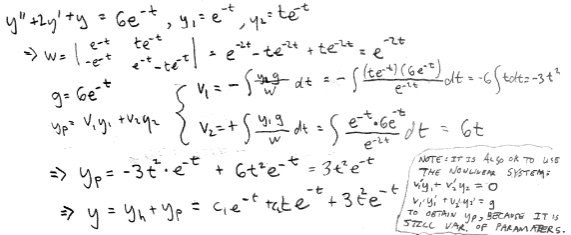
\includegraphics[width=16cm]{Images/ImgTest2VoP.jpg}
    \end{figure}  
} 
\else 
\vspace{3cm}
\fi
\fi


\ifnum \Version=2
\question[6] Consider the differential equation

    $$y'' + p(t)y' + q(t)y = 60t^3, \quad y=y(t)$$    
    
    Solutions to the corresponding homogeneous problem are $y_1 = 1$ and $y_2 = t^2$. 

    \begin{parts}
        \part Determine a particular solution to the differential equation using variation of parameters. Do not use the method of undetermined coefficients. 
        \ifnum \Solutions=0 
        \vspace{16cm}
        \fi
        \part State the general solution to the differential equation.
    \end{parts}
    \ifnum \Solutions=1 {\color{DarkBlue} 
    \begin{enumerate}
    \item[a)] The Wronskian is
\begin{align}
    W = \det \begin{pmatrix} 1&t^2\\0&2t\end{pmatrix} = 2t
\end{align}
To apply the formulas for the variation of parameters method for a second order DE we also use
\begin{align}
    y_1 & = 1 \\
    y_2 &= t^2 \\
    g &= 60t^3 
\end{align}
Applying the formulas for $v_1$ and $v_2$ we obtain
\begin{align}
    v_1 &= - \int \frac{y_2(t)g(t)}{W[y_1,y_2]}dt = - \int \frac{t^2 \cdot 60t^3}{2t} dt = - \int 30 t^4 \, dt = -6t^5 + k_1\\
    v_2 &= \int \frac{y_1(t)g(t)}{W[y_1,y_2]} dt = \int \frac{1\cdot60t^3}{2t} dt = \int 30 t^2 \, dt = 10t^3 + k_2
\end{align}
The arbitrary constants of integration, $k_1$ and $k_2$, in the above are actually not necessary. In the end they will only produce redundant terms because they are solutions to the homogeneous equation. But it is OK to leave them in the expressions for $v_1$ and $v_2$, in the expression for $y_p$, and the expression for $y$. The expression for $y_p$ becomes
\begin{align}
    y_p &= v_1y_1 + v_2y_2 \\
    &= (-6t^5 + k_1)\cdot 1 + (10t^3 + k_2) t^2 \\
    &= -6t^5 + k_1 + 10t^5 + k_2 t^2 \\
    &= 4t^5 + k_1 + k_2t^2
\end{align}
It is OK to ignore the terms with the integration constants and leave the solution as
\begin{align}
    y_p = v_1y_1 + v_2y_2 = -6t^5  + 10t^5 = 4t^5
\end{align}
\item [b)] The general solution to the differential equation is
\begin{align}
    y &= y_h + y_p \\
    &= c_1y_1 + c_2y_2 + v_1y_1 + v_2y_2 \\
    &= c_1 +c_2t^2 + 4t^5 + k_1  + k_2 t^2
\end{align}
Or we can write
\begin{align}
    y &= y_h + y_p  = c_1 +c_2t^2 + 4t^5 
\end{align}
\end{enumerate}
    } 
    \else 
    \fi    
\fi

\ifnum \Version=3
\question[6] Consider the differential equation

    $$y'' + p(t)y' + q(t)y = 60e^{-4t}, \quad y=y(t)$$    
    
    Solutions to the corresponding homogeneous problem are $y_1 = e^t$ and $y_2 = 1$. 
    
    \begin{parts}
        \part Determine a particular solution to the differential equation using variation of parameters. Do not use the method of undetermined coefficients. 
        \ifnum \Solutions=0 
        \vspace{16cm}
        \fi
        \part State the general solution to the differential equation.
    \end{parts}
    \ifnum \Solutions=1 {\color{DarkBlue}  
    \begin{enumerate}
    \item[a)] The Wronskian is
\begin{align}
    W = \det \begin{pmatrix} e^t&1\\e^t&0\end{pmatrix} = -e^t
\end{align}
The formulas for the variation of parameters method for a second order DE also uses:
\begin{align}
    y_1 & = e^t \\
    y_2 &= 1 \\
    g &= 60e^{-4t} 
\end{align}
Applying the formulas for $v_1$ and $v_2$ we obtain
\begin{align}
    v_1 &= - \int \frac{y_2(t)g(t)}{W[y_1,y_2]}dt 
    = - \int \frac{1 \cdot 60e^{-4t}}{-e^t} dt 
    = \int 60e^{-5t} \, dt 
    = -12e^{-5t} + k_1\\
    v_2 &= \int \frac{y_1(t)g(t)}{W[y_1,y_2]} dt 
    = \int \frac{e^t\cdot60e^{-4t}}{-e^t} dt 
    = - \int 60 e^{-4t}\, dt 
    = 15e^{-4t} + k_2
\end{align}
The arbitrary constants of integration, $k_1$ and $k_2$, in the above are actually not necessary. In the end they will only produce redundant terms because they are solutions to the homogeneous equation. But it is OK to leave them in the expressions for $v_1$ and $v_2$, in the expression for $y_p$, and the expression for $y$. 

The expression for $y_p$ becomes
\begin{align}
    y_p &= v_1y_1 + v_2y_2 \\
    &= (-12e^{-5t} + k_1)\cdot e^t + (15e^{-4t} + k_2) \cdot 1 \\
    &= 3e^{-4t} + k_1e^t + k_2
\end{align}
It is OK to ignore the terms with the integration constants and leave the solution as
\begin{align}
    y_p = v_1y_1 + v_2y_2 = 3e^{-4t}
\end{align}
\item [b)] The general solution to the differential equation is
\begin{align}
    y &= y_h + y_p \\
    &= c_1y_1 + c_2y_2 + v_1y_1 + v_2y_2 \\
    &= c_1e^t +c_2 + 3e^{-4t} + k_1e^t + k_2
\end{align}
Or we can write
\begin{align}
    y &= y_h + y_p  = c_1e^t +c_2 + 3e^{-4t} 
\end{align}
\end{enumerate}
    } 
    \else 
    \fi        
\fi


\ifnum \Version=4
\question[6] Consider the differential equation

    $$y'' + p(t)y' + q(t)y = 60t^3, \quad y=y(t)$$    
    
    Solutions to the corresponding homogeneous problem are $y_1 = 1$ and $y_2 = t^2$. 
    
    \begin{parts}
        \part Determine a particular solution to the differential equation using variation of parameters. Do not use the method of undetermined coefficients. 
        \ifnum \Solutions=0 
        \vspace{16cm}
        \fi
        \part State the general solution to the differential equation.
    \end{parts}
    \ifnum \Solutions=1 {\color{DarkBlue}  
    \begin{enumerate}
    \item[a)] The Wronskian is
\begin{align}
    W = \det \begin{pmatrix} 1&t^2\\0&2t\end{pmatrix} = 2t
\end{align}
To apply the formulas for the variation of parameters method for a second order DE we also use
\begin{align}
    y_1 & = 1 \\
    y_2 &= t^2 \\
    g &= 60t^3 
\end{align}
Applying the formulas for $v_1$ and $v_2$ we obtain
\begin{align}
    v_1 &= - \int \frac{y_2(t)g(t)}{W[y_1,y_2]}dt = - \int \frac{t^2 \cdot 60t^3}{2t} dt = - \int 30 t^4 \, dt = -6t^5 + k_1\\
    v_2 &= \int \frac{y_1(t)g(t)}{W[y_1,y_2]} dt = \int \frac{1\cdot60t^3}{2t} dt = \int 30 t^2 \, dt = 10t^3 + k_2
\end{align}
The arbitrary constants of integration, $k_1$ and $k_2$, in the above are actually not necessary. In the end they will only produce redundant terms because they are solutions to the homogeneous equation. But it is OK to leave them in the expressions for $v_1$ and $v_2$, in the expression for $y_p$, and the expression for $y$. The expression for $y_p$ becomes
\begin{align}
    y_p &= v_1y_1 + v_2y_2 \\
    &= (-6t^5 + k_1)\cdot 1 + (10t^3 + k_2) t^2 \\
    &= -6t^5 + k_1 + 10t^5 + k_2 t^2 \\
    &= 4t^5 + k_1 + k_2t^2
\end{align}
It is OK to ignore the terms with the integration constants and leave the solution as
\begin{align}
    y_p = v_1y_1 + v_2y_2 = -6t^5  + 10t^5 = 4t^5
\end{align}
\item [b)] The general solution to the differential equation is
\begin{align}
    y &= y_h + y_p \\
    &= c_1y_1 + c_2y_2 + v_1y_1 + v_2y_2 \\
    &= c_1 +c_2t^2 + 4t^5 + k_1  + k_2 t^2
\end{align}
Or we can write
\begin{align}
    y &= y_h + y_p  = c_1 +c_2t^2 + 4t^5 
\end{align}
\end{enumerate}
    } 
    \else 
    \fi
\fi

\ifnum \Version=5
\question[6] Consider the differential equation

    $$y'' + p(t)y' + q(t)y = 60e^{-4t}, \quad y=y(t)$$    
    
    Solutions to the corresponding homogeneous problem are $y_1 = e^t$ and $y_2 = 1$. 

    \begin{parts}
        \part Determine a particular solution to the differential equation using variation of parameters. Do not use the method of undetermined coefficients. 
        \ifnum \Solutions=0 
        \vspace{16cm}
        \fi
        \part State the general solution to the differential equation.
    \end{parts}
    \ifnum \Solutions=1 {\color{DarkBlue}  
    \begin{enumerate}
    \item[a)] The Wronskian is
\begin{align}
    W = \det \begin{pmatrix} e^t&1\\e^t&0\end{pmatrix} = -e^t
\end{align}
The formulas for the variation of parameters method for a second order DE also uses:
\begin{align}
    y_1 & = e^t \\
    y_2 &= 1 \\
    g &= 60e^{-4t} 
\end{align}
Applying the formulas for $v_1$ and $v_2$ we obtain
\begin{align}
    v_1 &= - \int \frac{y_2(t)g(t)}{W[y_1,y_2]}dt 
    = - \int \frac{1 \cdot 60e^{-4t}}{-e^t} dt 
    = \int 60e^{-5t} \, dt 
    = -12e^{-5t} + k_1\\
    v_2 &= \int \frac{y_1(t)g(t)}{W[y_1,y_2]} dt 
    = \int \frac{e^t\cdot60e^{-4t}}{-e^t} dt 
    = - \int 60 e^{-4t}\, dt 
    = 15e^{-4t} + k_2
\end{align}
The arbitrary constants of integration, $k_1$ and $k_2$, in the above are actually not necessary. In the end they will only produce redundant terms because they are solutions to the homogeneous equation. But it is OK to leave them in the expressions for $v_1$ and $v_2$, in the expression for $y_p$, and the expression for $y$. 

The expression for $y_p$ becomes
\begin{align}
    y_p &= v_1y_1 + v_2y_2 \\
    &= (-12e^{-5t} + k_1)\cdot e^t + (15e^{-4t} + k_2) \cdot 1 \\
    &= 3e^{-4t} + k_1e^t + k_2
\end{align}
It is OK to ignore the terms with the integration constants and leave the solution as
\begin{align}
    y_p = v_1y_1 + v_2y_2 = 3e^{-4t}
\end{align}
\item [b)] The general solution to the differential equation is
\begin{align}
    y &= y_h + y_p \\
    &= c_1y_1 + c_2y_2 + v_1y_1 + v_2y_2 \\
    &= c_1e^t +c_2 + 3e^{-4t} + k_1e^t + k_2
\end{align}
Or we can write
\begin{align}
    y &= y_h + y_p  = c_1e^t +c_2 + 3e^{-4t} 
\end{align}
\end{enumerate}
    } 
    \else 
    \fi    
\fi



\ifnum \Version>5
\question[4] Consider the first order system \[\vec{x} \, ' = \left( \begin{array}{rr} 2 & 4 \\ 4 & 2 \end{array} \right) \vec{x}  + \begin{pmatrix} 24\\0\end{pmatrix}  \]
    
    Solutions to the corresponding homogeneous problem are $\vec x_1 = e^{-2t}\begin{pmatrix} 1\\-1\end{pmatrix}$ and $\vec x_2 = e^{6t}\begin{pmatrix} 1\\1\end{pmatrix}$. 

    \begin{parts}
        \part Determine a particular solution to the differential equation using variation of parameters. Do not use the method of undetermined coefficients. 
\ifnum \Solutions=0 \vspace{17cm}\fi
        \part State the general solution to the system of differential equations. 
    \end{parts}
    \ifnum \Solutions=1 {\color{DarkBlue}   
    
    \begin{itemize}
        \item \textbf{Fundamental Matrix}\\
        The fundamental matrix \(X(t)\) is constructed by placing the solutions \(\vec{x}_1\) and \(\vec{x}_2\) as columns in a matrix. Thus,
        
        \[
        X(t) = \begin{pmatrix} \vec{x}_1 & \vec{x}_2 \end{pmatrix} = \begin{pmatrix} e^{-2t} & e^{6t} \\ -e^{-2t} & e^{6t} \end{pmatrix}
        \]
        \item \textbf{Inverse}\\
        \begin{align*}
            \det(X(t)) &= e^{-2t} \cdot e^{6t} - e^{6t} \cdot (-e^{-2t}) = e^{4t} + e^{4t} = 2e^{4t}\\
            X^{-1} &= \frac{1}{2e^{4t}} \begin{pmatrix} e^{6t} & -e^{6t} \\ e^{-2t} & e^{-2t} \end{pmatrix}
        = \frac{1}{2} \begin{pmatrix} e^{2t} & -e^{2t} \\ e^{-6t} & e^{-6t} \end{pmatrix}
        \end{align*}
        
        \item \textbf{Particular}\\
        \begin{align}
            \vec x_p &= X \int X^{-1} g \, dt \\
            &= X \int \frac{1}{2} \begin{pmatrix} e^{2t} & -e^{2t} \\ e^{-6t} & e^{-6t} \end{pmatrix} \begin{pmatrix} 24 \\ 0 \end{pmatrix} \, dt \\
            & = X \int \begin{pmatrix} 12e^{2t} \\ 12e^{-6t} \end{pmatrix} \, dt \\
            &= \begin{pmatrix} e^{-2t} & e^{6t} \\ -e^{-2t} & e^{6t} \end{pmatrix} \begin{pmatrix} 6e^{2t} + C_1 \\ -2e^{-6t} + C_2 \end{pmatrix} \\
            &=  \begin{pmatrix} 4 + C_1 e^{-2t} + C_2 e^{6t} \\ -8 - C_1 e^{-2t} + C_2 e^{6t} \end{pmatrix}
        \end{align}  
        It is not necessary to keep the $C_1$ and $C_2$ terms, they can be ignored. 
        \item \textbf{General Solution}
        \begin{align}
            \vec x = \vec x_h + \vec x_p = c_1 e^{-2t}\begin{pmatrix} 1\\-1\end{pmatrix} + c_2 e^{6t}\begin{pmatrix} 1\\1\end{pmatrix} + \begin{pmatrix} 4\\-8\end{pmatrix}
        \end{align}

    \end{itemize}




    } 
    \else 
    \fi    
\fi

 
        \ifnum \Version=4
            \renewcommand{\Version}{2}
        \fi
        \ifnum \Version=5
            \renewcommand{\Version}{3}
        \fi        
        \ifnum \Solutions=0
\newpage 
\fi
\ifnum \Version=1
    \question[5] Consider the non-linear system below.  
    \begin{align*}
        \dxdt &= y(x+y-6) , \qquad \dydt = x(2x+y-8)
    \end{align*}
    \begin{parts}
        \part Determine the locations of the critical points. 
        \ifnum \Solutions=1 {\color{DarkBlue} \\[12pt] 
        Setting both $x'=0$ and $y'=0$, we obtain four critical points as follows. $x'=0$ implies $y=0$ or $x+y-6=0$. 
            \begin{itemize}
                \item If $y=0$, then for $y'=0$ we need either $x=0$ or $2x+y-8=0$. 
                \begin{itemize}
                    \item If $y=0$ and $x=0$, one critical point is at $(0,0)$. 
                    \item If $y=0$ and $2x+y-8=0$, one critical point is at $(4,0)$. 
                \end{itemize}
                \item If $x+y-6=0$, then for $y'=0$ we need either $x=0$ or $2x+y-8=0$. 
                \begin{itemize}
                    \item If $x+y-6=0$ and $x=0$, one critical point is at $(0,6)$. 
                    \item If $x+y-6=0$ and $2x+y-8=0$, then solving this system of equations yields a critical point at $(2,4)$. 
                \end{itemize}                
            \end{itemize}
            The four critical points are located at $(0,0)$, $(4,0)$, $(0,6)$, $(2,4)$. 
            } 
        \else 
        \vfill
        \fi
        \part Sketch the nullclines of the system on the axes below. Clearly indicate the critical points that you found in part (a). 
        \ifnum \Solutions=1 {\color{DarkBlue} \\[12pt] 
        Green lines are the $x-$nullclines, red lines are the $y-$nullclines.
        \begin{center}
        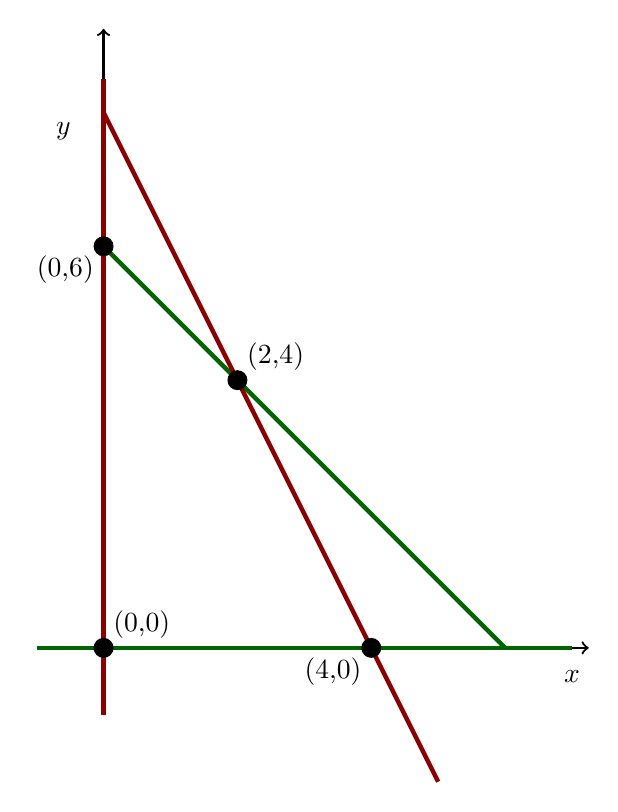
\begin{tikzpicture}[scale=0.85]
        \draw[thick, ->] (-1, 0) -- (7.25, 0);
        \draw[thick, ->] (0, -1) -- (0, 9.25);
        \node[overlay, below] at (7, -0.2) {$x$};
        \node[overlay, below] at (-0.6, 8) {$y$};   
        \draw[ultra thick,DarkGreen, -] (-1, 0) -- (7, 0);        
        \draw[ultra thick,DarkGreen, -] (0,6) -- (6, 0);   
        \draw[ultra thick,DarkRed, -] (0, 8) -- (5, -2);        
        \draw[ultra thick,DarkRed, -] (0, -1) -- (0, 8.5);      
        \filldraw[black] (0,0) circle (4pt) node[anchor=south west]{(0,0)};
        \filldraw[black] (0,6) circle (4pt) node[anchor=north east]{(0,6)};
        \filldraw[black] (2,4) circle (4pt) node[anchor=south west]{(2,4)};
        \filldraw[black] (4,0) circle (4pt) node[anchor=north east]{(4,0)};
        \end{tikzpicture}
        \end{center}            
        } 
        \else 
        \begin{center}
        \begin{tikzpicture}[scale=0.55]
        \draw[very thick, ->] (-6, 0) -- (6.25, 0);
        \draw[very thick, ->] (0, -6) -- (0, 6.25);
        \node[overlay, below] at (6, -0.2) {$x$};
        \node[overlay, below] at (-0.6, 6) {$y$};        
        \end{tikzpicture}
        \end{center}    
    \fi
    \end{parts}
\fi 





\ifnum \Version=2
    \question[6] Consider the non-linear system below.  
    \begin{align*}
        \dxdt &= (x-1)(y-5) , \qquad \dydt = y-x^2-1
    \end{align*}
    \begin{parts}
        \part Determine the locations of the critical points. 
        \ifnum \Solutions=1 {\color{DarkBlue} \\[12pt] 
        For a point to be a critical point, we need $x' = y' = 0$. If $x'$ is zero, then either $x=1$ or $y=5$. 
        \begin{itemize}
            \item When $x=1$, for $y'=0$ we need 
            \begin{align}
                y'&=0 = y - x^2 - 1 \quad \Rightarrow \quad y = 1^2+1 = 2
            \end{align}
            There is a critical point at $(1,2)$. 
            \item When $y=5$, for $y'=0$ we need 
            \begin{align}
                y'&=0 = y - x^2 - 1 \quad \Rightarrow \quad x^2 = 5 - 1 \quad \Rightarrow \quad x = \pm 2
            \end{align}
            There are critical points at $(\pm 2, 5)$.             
        \end{itemize}
            } 
        \else 
        \vfill
        \fi
        \part Sketch the nullclines of the system on the axes below. Clearly indicate the critical points that you found in part (a). 
        \ifnum \Solutions=1 {\color{DarkBlue} \\[12pt] 
        The curves are shown below. The green lines are the x nullclines, and the red curve is the y nullcline. There are exactly three critical points. 
            \begin{center}
            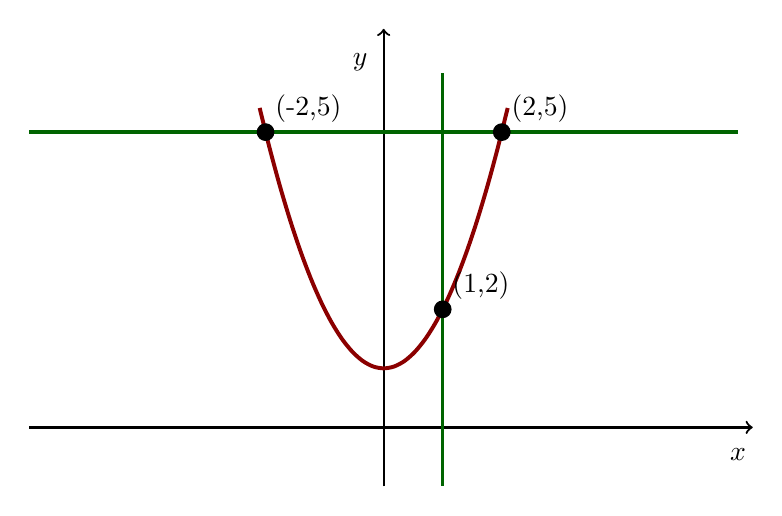
\begin{tikzpicture}[scale=0.75]
            \draw[thick, ->] (-6, 0) -- (6.25, 0);
            \draw[thick, ->] (0, -1) -- (0, 6.75);
            \node[overlay, below] at (6, -0.2) {$x$};
            \node[overlay, below] at (-0.4, 6.5) {$y$};   
            \draw[very thick,DarkGreen, -] (1, 6) -- (1, -1);        
            \draw[very thick,DarkGreen, -] (-6, 5) -- (6, 5);   
            \draw[DarkRed, line width = 0.50mm]   plot[smooth,domain=-2.1:2.1] (\x, {\x*\x+1});
            \filldraw[black] (2,5) circle (4pt) node[anchor=south west]{(2,5)};
            \filldraw[black] (-2,5) circle (4pt) node[anchor=south west]{(-2,5)};
            \filldraw[black] (1,2) circle (4pt) node[anchor=south west]{(1,2)};
            \end{tikzpicture}
            \end{center}               
        } 
        \else 
        \begin{center}
        \begin{tikzpicture}[scale=0.55]
        \draw[very thick, ->] (-6, 0) -- (6.25, 0);
        \draw[very thick, ->] (0, -6) -- (0, 6.25);
        \node[overlay, below] at (6, -0.2) {$x$};
        \node[overlay, below] at (-0.6, 6) {$y$};        
        \end{tikzpicture}
        \end{center}    
    \fi
    \end{parts}
\fi 




\ifnum \Version=3
    \question[6] Consider the non-linear system below.  
    \begin{align*}
        \dxdt &= (x-1)(y-2) , \qquad \dydt = y^2-x
    \end{align*}
    \begin{parts}
        \part Determine the locations of the critical points. 
        \ifnum \Solutions=1 {\color{DarkBlue} \\[12pt] 
        For a point to be a critical point, we need $x' = y' = 0$. If $x'$ is zero, then either $x=1$ or $y=2$. 
        \begin{itemize}
            \item When $x=1$, for $y'=0$ we need 
            \begin{align}
                y'&=0 = y^2 - x \quad \Rightarrow \quad y = \pm 1
            \end{align}
            There are critical points at $(1,\pm 1)$. 
            \item When $y=2$, for $y'=0$ we need 
            \begin{align}
                y'&=0 = y^2 - x  \quad \Rightarrow \quad x = 4 
            \end{align}
            There is a critical point at $(4, 2)$.             
        \end{itemize}
            } 
        \else 
        \vfill
        \fi
        \part Sketch the nullclines of the system on the axes below. Clearly indicate the critical points that you found in part (a). 
        \ifnum \Solutions=1 {\color{DarkBlue} \\[12pt] 
        The curves are shown below. The green lines are the x nullclines, and the red curve is the y nullcline. There are exactly three critical points. 
            \begin{center}
            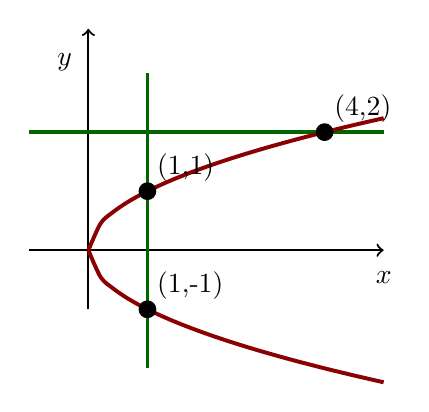
\begin{tikzpicture}[scale=0.75]
            \draw[thick, ->] (-1, 0) -- (5, 0);
            \draw[thick, ->] (0, -1) -- (0, 3.75);
            \node[overlay, below] at (5, -0.2) {$x$};
            \node[overlay, below] at (-0.4, 3.5) {$y$};   
            \draw[very thick,DarkGreen, -] (1, 3) -- (1, -2);        
            \draw[very thick,DarkGreen, -] (-1, 2) -- (5, 2);   
            \draw[DarkRed, line width = 0.50mm]   plot[smooth,domain=0:5] (\x, {\x^(1/2))} );
            \draw[DarkRed, line width = 0.50mm]   plot[smooth,domain=0:5] (\x, {-\x^(1/2))} );
            \filldraw[black] (4,2) circle (4pt) node[anchor=south west]{(4,2)};
            \filldraw[black] (1,1) circle (4pt) node[anchor=south west]{(1,1)};
            \filldraw[black] (1,-1) circle (4pt) node[anchor=south west]{(1,-1)};
            \end{tikzpicture}
            \end{center}               
        } 
        \else 
        \begin{center}
        \begin{tikzpicture}[scale=0.55]
        \draw[very thick, ->] (-6, 0) -- (6.25, 0);
        \draw[very thick, ->] (0, -6) -- (0, 6.25);
        \node[overlay, below] at (6, -0.2) {$x$};
        \node[overlay, below] at (-0.6, 6) {$y$};        
        \end{tikzpicture}
        \end{center}    
    \fi
    \end{parts}
\fi 


\ifnum \Version=6
    \question[4] Consider the non-linear system below.  
    \begin{align*}
        \dxdt &= (x-2)(y-1) , \qquad \dydt = 2y^2-x
    \end{align*}
    \begin{parts}
        \part Determine the locations of the critical points. 
        \ifnum \Solutions=1 {\color{DarkBlue} \\[12pt] 
        For a point to be a critical point, we need $x' = y' = 0$. If $x'$ is zero, then either $x=2$ or $y=1$. 
        \begin{itemize}
            \item When $x=2$, for $y'=0$ we need 
            \begin{align}
                y'&=0 = 2y^2 - x \quad \Rightarrow \quad y = \pm 1
            \end{align}
            There are critical points at $(2,\pm 1)$. 
            \item When $y=1$, for $y'=0$ we need 
            \begin{align}
                y'&=0 = 2y^2 - x  \quad \Rightarrow \quad x = 2
            \end{align}
            There is a critical point at $(2,1)$, which we already had.          
        \end{itemize}
            } 
        \else 
        \vfill
        \fi
        \part Sketch the nullclines of the system on the axes below. Clearly indicate the critical points that you found in part (a). 
        \ifnum \Solutions=1 {\color{DarkBlue} \\[12pt] 
        The curves are shown below. The green lines are the x nullclines, and the red curve is the y nullcline. There are exactly three critical points. 
            \begin{center}
            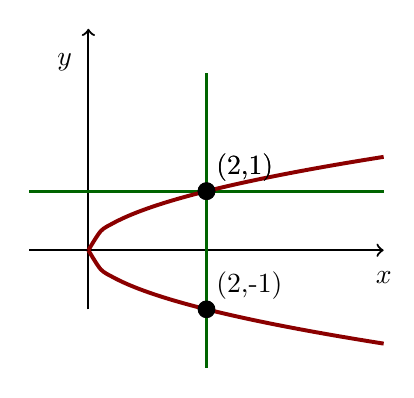
\begin{tikzpicture}[scale=0.75]
            \draw[thick, ->] (-1, 0) -- (5, 0);
            \draw[thick, ->] (0, -1) -- (0, 3.75);
            \node[overlay, below] at (5, -0.2) {$x$};
            \node[overlay, below] at (-0.4, 3.5) {$y$};   
            \draw[very thick,DarkGreen, -] (2, 3) -- (2, -2);        
            \draw[very thick,DarkGreen, -] (-1, 1) -- (5, 1);   
            \draw[DarkRed, line width = 0.50mm]   plot[smooth,domain=0:5] (\x, {(\x/2)^(1/2))} );
            \draw[DarkRed, line width = 0.50mm]   plot[smooth,domain=0:5] (\x, {-(\x/2)^(1/2))} );
            \filldraw[black] (2,1) circle (4pt) node[anchor=south west]{(2,1)};
            \filldraw[black] (2,1) circle (4pt) node[anchor=south west]{(2,1)};
            \filldraw[black] (2,-1) circle (4pt) node[anchor=south west]{(2,-1)};
            \end{tikzpicture}
            \end{center}               
        } 
        \else 
        \begin{center}
        \begin{tikzpicture}[scale=0.55]
        \draw[very thick, ->] (-6, 0) -- (6.25, 0);
        \draw[very thick, ->] (0, -6) -- (0, 6.25);
        \node[overlay, below] at (6, -0.2) {$x$};
        \node[overlay, below] at (-0.6, 6) {$y$};        
        \end{tikzpicture}
        \end{center}    
    \fi
    \end{parts}
\fi 


\ifnum \Version=7
    \question[4] Consider the non-linear system below.  
    \begin{align*}
        \dxdt &= (x-1)(y-5) , \qquad \dydt = y-x^2-1
    \end{align*}
    \begin{parts}
        \part Determine the locations of the critical points. 
        \ifnum \Solutions=1 {\color{DarkBlue} \\[12pt] 
        For a point to be a critical point, we need $x' = y' = 0$. If $x'$ is zero, then either $x=1$ or $y=5$. 
        \begin{itemize}
            \item When $x=1$, for $y'=0$ we need 
            \begin{align}
                y'&=0 = y - x^2 - 1 \quad \Rightarrow \quad y = 1^2+1 = 2
            \end{align}
            There is a critical point at $(1,2)$. 
            \item When $y=5$, for $y'=0$ we need 
            \begin{align}
                y'&=0 = y - x^2 - 1 \quad \Rightarrow \quad x^2 = 5 - 1 \quad \Rightarrow \quad x = \pm 2
            \end{align}
            There are critical points at $(\pm 2, 5)$.             
        \end{itemize}
            } 
        \else 
        \vfill
        \fi
        \part Sketch the nullclines of the system on the axes below. Clearly indicate the critical points that you found in part (a). 
        \ifnum \Solutions=1 {\color{DarkBlue} \\[12pt] 
        The curves are shown below. The green lines are the x nullclines, and the red curve is the y nullcline. There are exactly three critical points. 
            \begin{center}
            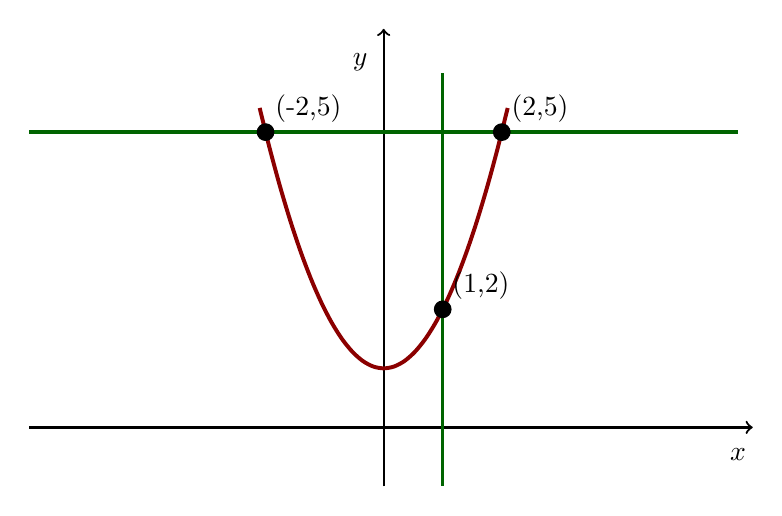
\begin{tikzpicture}[scale=0.75]
            \draw[thick, ->] (-6, 0) -- (6.25, 0);
            \draw[thick, ->] (0, -1) -- (0, 6.75);
            \node[overlay, below] at (6, -0.2) {$x$};
            \node[overlay, below] at (-0.4, 6.5) {$y$};   
            \draw[very thick,DarkGreen, -] (1, 6) -- (1, -1);        
            \draw[very thick,DarkGreen, -] (-6, 5) -- (6, 5);   
            \draw[DarkRed, line width = 0.50mm]   plot[smooth,domain=-2.1:2.1] (\x, {\x*\x+1});
            \filldraw[black] (2,5) circle (4pt) node[anchor=south west]{(2,5)};
            \filldraw[black] (-2,5) circle (4pt) node[anchor=south west]{(-2,5)};
            \filldraw[black] (1,2) circle (4pt) node[anchor=south west]{(1,2)};
            \end{tikzpicture}
            \end{center}               
        } 
        \else 
        \begin{center}
        \begin{tikzpicture}[scale=0.55]
        \draw[very thick, ->] (-6, 0) -- (6.25, 0);
        \draw[very thick, ->] (0, -6) -- (0, 6.25);
        \node[overlay, below] at (6, -0.2) {$x$};
        \node[overlay, below] at (-0.6, 6) {$y$};        
        \end{tikzpicture}
        \end{center}    
    \fi
    \end{parts}
\fi 

        \ifnum \Solutions=0
\newpage 
\fi
\ifnum \Version=1
\question[5] Consider the non-linear system below.  
\begin{align*}
    \dxdt &= x^2+y-2x-12 , \qquad \dydt = y-x-6
\end{align*}
The critical points are located at $(-2,4)$ and $(3,9)$. 
\begin{parts}
    \part Compute the Jacobian matrix, $J$, for the approximating linear system. 
    \ifnum \Solutions=1 {\color{DarkBlue}
        \begin{align}
            F &= x'\\
            G &= y' \\
            J &= \begin{pmatrix} F_x&F_y\\ G_x & G_y\end{pmatrix} = \begin{pmatrix} 2x-2&1\\-1&1\end{pmatrix}
        \end{align}
        } 
    \else 
    \vfill
    \fi        
    \part Use eigenvalues to classify the critical point at $(-2,4)$ according to stability (stable, unstable, asymptotically stable) and type (saddle, proper node, etc).
    \ifnum \Solutions=1 {\color{DarkBlue} \\[12pt] 
        At $(-2,4)$, $J = \begin{pmatrix} -6&1\\-1&1\end{pmatrix}$. The eigenvalues are the roots of \begin{align}
            (-6-\lambda)(1-\lambda)+1 = \lambda^2 +5\lambda - 5
        \end{align}
        Thus 
        \begin{align}
            \lambda = -\frac52 \pm \frac12 \sqrt{25-4\cdot(-5)} = -\frac52 \pm \frac{\sqrt{45}}{2}
        \end{align}
        $\lambda \in \mathbb R$, and the eigenvalues have opposite signs. The critical point is an unstable saddle. 
        } 
    \else 
    \vfill
    \fi
    \part Use eigenvalues to classify the critical point at $(3,9)$ according to stability (stable, unstable, asymptotically stable) and type (saddle, proper node, etc).
    \ifnum \Solutions=1 {\color{DarkBlue} \\[12pt] 
        At $(3,9)$, $J = \begin{pmatrix} 4&1\\-1&1\end{pmatrix}$. The eigenvalues are the roots of \begin{align}
            (4-\lambda)(1-\lambda)+1 = \lambda^2 - 5\lambda +5 
        \end{align}
        Thus 
        \begin{align}
            \lambda = \frac52 \pm \frac12 \sqrt{25-4\cdot(5)} = \frac52 \pm \frac{\sqrt{5}}{2}
        \end{align}
        $\lambda \in \mathbb R$, and the eigenvalues both positive. The critical point is an unstable node. 
    } 
    \else 
    \vfill
\fi
\end{parts}
\fi



\ifnum \Version=2
\question[6] Consider the non-linear system below.  
\begin{align*}
    \dxdt &= x(1-x-y) , \qquad \dydt = y(2-x-y)
\end{align*}
The critical points are located at $(0,0)$, $(0,2)$, and $(1,0)$. 
\begin{parts}
    \part Compute the Jacobian matrix, $J$, for the approximating linear system. 
    \ifnum \Solutions=1 {\color{DarkBlue} \\
    Set $ F = x'$ and $G = y'$. Then
        \begin{align}
            F_x &= 1 - 2x -y\\
            F_y &= -x \\
            G_x &= 2-x-2y \\
            G_y &= -y \\
            J &= \begin{pmatrix} F_x&F_y\\ G_x & G_y\end{pmatrix} = \begin{pmatrix} -1-x-2y & -x\\-y&2-x-2y \end{pmatrix}
        \end{align}
        } 
    \else 
    \vfill
    \fi        
    \part Use eigenvalues to classify the critical point at $(0,0)$ according to stability (stable, unstable, asymptotically stable) and type (saddle, proper node, etc).
    \ifnum \Solutions=1 {\color{DarkBlue} \\[12pt] 
        At $(0,0)$, $J = \begin{pmatrix} 1&0\\0&2\end{pmatrix}$. The eigenvalues are $\lambda = 1,2$. \\ Thus the critical point is an \textbf{unstable node}. 
        } 
    \else 
    \vfill
    \fi
    \part Use eigenvalues to classify the critical point at $(0,2)$ according to stability (stable, unstable, asymptotically stable) and type (saddle, proper node, etc).
    \ifnum \Solutions=1 {\color{DarkBlue} \\[12pt] 
        At $(0,2)$, $J = \begin{pmatrix} -1&0\\-2&-4\end{pmatrix}$. The eigenvalues are $\lambda = -1,-4$. \\Thus the critical point is a \textbf{stable node}. 
        } 
    \else 
    \vfill
    \fi
    \part Use eigenvalues to classify the critical point at $(1,0)$ according to stability (stable, unstable, asymptotically stable) and type (saddle, proper node, etc).
    \ifnum \Solutions=1 {\color{DarkBlue} \\[12pt] 
        At $(1,0)$, $J = \begin{pmatrix} -1&-1\\0&1\end{pmatrix}$. The eigenvalues are $\lambda = \pm 1$. \\ Thus the critical point is an \textbf{unstable saddle}. 
        } 
    \else 
    \vfill
    \fi    
\end{parts}
\fi










\ifnum \Version>5
\question[6] Consider the non-linear system below.  
\begin{align*}
    \dxdt &= x(4-x-y) , \qquad \dydt = y(6-2x-y)
\end{align*}
\begin{parts}
    \part Compute the Jacobian matrix, $J$, for the approximating linear system. 
    \ifnum \Solutions=1 {\color{DarkBlue} \\
    Set $ F = x'$ and $G = y'$. Then
        \begin{align}
            F &= 4x - x^2 - xy \\
            G &= 6y -2xy - y^2 \\
            J &= \begin{pmatrix} F_x&F_y\\ G_x & G_y\end{pmatrix} 
            = \begin{pmatrix} 4-2x-y & -x\\-2y& 6-2x-2y \end{pmatrix}
        \end{align}
        } 
    \else 
    \vfill
    \fi        
    \part Use eigenvalues to classify the critical point at $(0,6)$ according to stability (stable, unstable, asymptotically stable) and type (saddle, proper node, etc).
    \ifnum \Solutions=1 {\color{DarkBlue} \\[12pt] 
        At $(0,0)$, $J = \begin{pmatrix} -2&0\\-12&-6\end{pmatrix}$. The eigenvalues are $\lambda = -2, -6$. The CP is a \textbf{stable node}. 
        } 
    \else 
    \vfill
    \fi
    \part Use eigenvalues to classify the critical point at $(2,2)$ according to stability (stable, unstable, asymptotically stable) and type (saddle, proper node, etc).
    \ifnum \Solutions=1 {\color{DarkBlue} \\[12pt] 
        At $(0,2)$, $J = \begin{pmatrix} -2&-2\\-4&-2\end{pmatrix}$. Eigenvalues:
        \begin{align}
            0 &= (\lambda + 2)^2 - 8 = \lambda^2 + 4\lambda -4  \\
            \lambda &= -2 \pm \frac12 \sqrt{16 + 16} = -2 \pm 2\sqrt 2
        \end{align}\\Thus the critical point is an \textbf{unstable saddle}. 
        } 
    \else 
    \vfill
    \fi
\end{parts}
\fi


        \ifnum \Solutions=0
\newpage 
\fi
\ifnum \Version=1    
    \question[6] Use the Laplace transform to solve the following IVP. Do not leave your answer in terms of an integral. Please show your work.
    % $$\displaystyle y''-4y'+4y=0,\qquad y(0)=1,\quad y'(0)=1$$ %Q,A HW 5.4#4
    % $$\displaystyle y''-2y'+4y=0,\qquad y(0)=2,\quad y'(0)=0$$ %M HW 5.4#5
    $$ y'' -6y'+13y = 0, \quad y(0) = 0, \quad y'(0) = -3$$. % A TRIM P301 #27
    % $$ y''+ 2y'+y = 0, \quad y(0) = 1, \quad y'(0) = 1$$. % B TRIM P301 #23
\ifnum \Solutions=1 {\color{DarkBlue} 
Take the transform of the DE and solve for $Y(s) = \mathcal{L}[y(t)]$.
\begin{align}
    0
    &= s^2Y-sy(0) - y'(0) - 6(sY-y(0)) + 13Y \\
    &= s^2Y-0 +3 - 6(sY-0) + 13Y \\
    -3 &= s^2Y - 6sY + 13Y \\
    -3 &= (s^2 - 6s + 13)Y \\
    Y &= \frac{-3}{s^2- 6s+13} 
\end{align}    
Complete the square:
\begin{align}
    Y &= \frac{-3}{s^2- 6s+9-9+13} = \frac{-3}{ (s-3)^2+4}=\frac{-3}{2}\cdot \frac{2}{ (s-3)^2+4}
\end{align}    
Inverse transform:
\begin{align}
    y(t) &= \frac{-3}{2}\sin(2t)e^{3t}
\end{align}
} 
\else 
\vspace{3cm}
\fi
\fi 



\ifnum \Version=2
    \question[6] Consider the IVP: $y''+4y'+3y = 4e^{-2t}$, $y(0)=0, y'(0) = 0$. 
        \begin{parts}
        \part Use the Laplace Transform to obtain an explicit expression for $Y(s) = \mathcal{L}[y]$. 
        \ifnum \Solutions=1 {\color{DarkBlue} \\[12pt] 
        Taking the transform of the IVP yields
        \begin{align}
            s^2Y-sy(0) - y'(0) +4(sY-y(0)) +3 Y &= \frac{4}{s+2} \\
            (s^2 +4s+3)Y &= \frac{4}{s+2} \\
            Y&= \frac{1}{s+2} \frac{4}{s^2 +4s+3} \\
            &= \frac{4}{(s+1)(s+2)(s+3)}
        \end{align}
        } 
        \else 
        \vfill
        \fi
        \part Use the inverse Laplace Transform to solve the IVP. 
        \ifnum \Solutions=1 {\color{DarkBlue} \\[12pt] 
        Partial fractions: 
        \begin{align}
            \frac{4}{(s+2)(s+1)(s+3)} & = \frac{A}{s+1} + \frac{B}{s+2} + \frac{C}{s+3} \\
            4 & = A(s+2)(s+3) + B(s+1)(s+3) + C(s+1)(s+2) 
        \end{align}
        Selecting values of $s$ yields
        \begin{align}
            s=-1: \quad 4 & = 2A + 0 + 0 \quad \Rightarrow \quad A = 2 \\
            s=-2: \quad 4 & = 0 - B + 0 \quad \Rightarrow \quad B = -4 \\
            s=-3: \quad 4 & = 0 + 0 + 2C \quad \Rightarrow \quad C = 2
        \end{align}
        Thus
       \begin{align}
            Y (s) = \frac{4}{(s+1)(s+2)(s+3)} 
            &= \frac{A}{s+1} + \frac{B}{s+2} + \frac{C}{s+3} \\
            &= \frac{2}{s+1} + \frac{-4}{s+2} + \frac{2}{s+3} 
        \end{align}        
        With the inverse transform this becomes 
        \begin{align}
            y(t) &= 2e^{-t} -4 e^{-2t} +2 e^{-3t}
        \end{align}
        } 
        \else 
        \vfill
        \fi
    \end{parts}
\fi 




\ifnum \Version>5
    \question[4] Consider the IVP: $y''+4y = 8e^{-2t}$, $y(0)=0, y'(0) = 0$. 
        \begin{parts}
        \part Use the Laplace Transform to obtain an explicit expression for $Y(s) = \mathcal{L}[y]$. 
        \ifnum \Solutions=1 {\color{DarkBlue} \\[12pt] 
        Taking the transform of the IVP yields
        \begin{align}
            s^2Y-sy(0) - y'(0) + 4 Y &= \frac{8}{s+2} \\
            (s^2 + 4)Y &= \frac{8}{s+2} \\
            Y&= \frac{8}{s+2} \frac{1}{s^2 + 4} \\
            &= \frac{8}{(s^2+4)(s+2)}
        \end{align}
        } 
        \else 
        \vfill
        \fi
        \part Use the inverse Laplace Transform to solve the IVP. 
        \ifnum \Solutions=1 {\color{DarkBlue} \\[12pt] 
        Partial fractions: 
        \begin{align}
            \frac{8}{(s^2+4)(s+2)} & = \frac{As+B}{s^2+4} + \frac{C}{s+2} \\
            8 & = (As+B)(s+2) + C(s^2+4) \\
            8 &= (A+C)s^2 +(2A+B)s+(2B+4C)
        \end{align}
        Selecting $s = -2$ yields
        \begin{align}
            s=-2: \quad 8 & = 0 + C((-2)^2+4) \quad \Rightarrow \quad C = 1 
        \end{align}
        The quadratic terms give us 
        \begin{align}
            A+C = 0 \Rightarrow \quad A = - 1 
        \end{align}
        The linear terms give us 
        \begin{align}
            2A+B = 0 \Rightarrow \quad B = 2
        \end{align}        
        Thus
       \begin{align}
            Y (s) = \frac{8}{(s^2+4)(s+2)} 
            &= \frac{As+B}{s^2+4} + \frac{C}{s+2} \\
            &= \frac{-s+2}{s^2+4} + \frac{1}{s+2} \\
            &= -\frac{s}{s^2+4} + \frac{2}{s^2+4} + \frac{1}{s+2} \\
        \end{align}        
        With the inverse transform this becomes 
        \begin{align}
            y(t) &= \sin(2t) - \cos(2t) + e^{-2t}
        \end{align}
        \textbf{Additional Notes}\\
        Some students made an error in taking the transform that resulted in the expression
        $$Y = \frac{8}{s(s+4)(s+2)} = \frac1s+\frac{1}{s+4}- \frac{2}{s+2}$$
        } 
        \else 
        \vfill
        \fi
    \end{parts}
\fi 


        \ifnum \Solutions=0
\newpage 
\fi

\ifnum \Version=1    
\question[2] 
Compute the Laplace transform of the function below. Do not leave your answer in terms of an integral. Please show your work. 
$$y(t) = \begin{cases} 0, \quad 0 \le t < 1 \\ t-2, \quad 1 \le t < 3 \\ 0, \quad 3 \le t < \infty\end{cases}$$
\ifnum \Solutions=1 {\color{DarkBlue} \\[12pt] 
There are a few different ways to solve this. Any of the approaches below are sufficient. 
\subsection*{Method 1: Direct Integration }
Direct integration requires integration by parts, but using the definition of the Laplace Transform:
    \begin{align}
        \int_0^{\infty} e^{-st} y(t) \, dt 
        &= \int_1^{3} e^{-st} \, (t-2) \, dt \\
        &= \int_1^{3} te^{-st}  \, dt - 2 \int_1^{3} e^{-st}  \, dt \\
        &=  \left. t\cdot \frac{-1}{s}e^{-st} \right|_1^3
        - \int_1^{3} \frac{-1}{s}e^{-st} \, dt 
        -2 \left( \left. \frac{-1}{s}e^{-st}\right|_{t=1}^{t=3}\right) \\
        &=  \frac{-1}{s}\left( 3e^{-3s} - e^{-s} \right)  
        + \frac{1}{s} \int_1^{3} e^{-st} \, dt 
        + \frac{2}{s} \left(  e^{-3s} - e^{-s} \right) \\
        &=  \frac{-1}{s}\left( 3e^{-3s} - e^{-s} \right)  
        + \frac{1}{s} \left( \left. \frac{-1}{s}e^{-st}\right|_{t=1}^{t=3}\right) \, dt 
        + \frac{2}{s} \left(  e^{-3s} - e^{-s} \right) \\     
        &=  \frac{-1}{s}\left( 3e^{-3s} - e^{-s} \right)  
        - \frac{1}{s^2} \left(  e^{-3s} - e^{-s} \right) 
        + \frac{2}{s} \left(  e^{-3s} - e^{-s} \right) \\      
        &= - \frac{1}{s^2} \left(  e^{-3s} - e^{-s} \right) 
        - \frac{ e^{-3s}}{s}   - \frac{e^{-s}}{s}  \\   
        &= \frac{e^{-s}}{s^2} - \frac{e^{-3s}}{s^2} 
        - \frac{ e^{-3s}}{s}   - \frac{e^{-s}}{s}           
    \end{align}
    \subsection*{Method 2: Step Functions}
    We could also use the table of transforms, specifically the transform of the step function $u_c(t)$ and its product with another function. 
    \begin{align}
        y(t) &= 0u_{0,1} + (t-2)u_{1,3} + 0u_{3} 
        =(t-2)(u_1-u_3) 
        = tu_1-tu_3 - 2u_1 + 2 u_3 
    \end{align}   
    At this point we can either take the transform and use the derivative theorem (in the table) to work out the transform of $tu_1$ and $tu_3$, or we can use the following trick:
    \begin{align}
        y(t) &= tu_1-tu_3 - 2u_1 + 2 u_3 \\
        &= (t+1-1)u_1-(t+3-3)u_3 - 2u_1 + 2 u_3 \\
        &= (t-1)u_1 + u_1 -(t-3)u_3 - 3u_3 - 2u_1 + 2 u_3 \\
        &= (t-1)u_1 -(t-3)u_3 - u_1 - u_3 
    \end{align}
    Using the table of transforms the Laplace transform is
    \begin{align}
        Y(s) = \frac{e^{-s}}{s^2} - \frac{e^{-3s}}{s^2} - \frac{e^{-s}}{s} - \frac{e^{-3s}}{s}
    \end{align}
} 
\else 
    \vfill
    \begin{center}
        \textit{This remainder of this page can be used for scratch work. }
    \end{center}
    \vfill
\fi
\fi


\ifnum \Version=5
\question[2] 
Compute the Laplace transform of the function below. Do not leave your answer in terms of an integral. Please show your work. 
$$y(t) = \begin{cases} 0, \quad 0 \le t < 1 \\ 4, \quad 1 \le t < 3 \\ 0, \quad 3 \le t < \infty\end{cases}$$
\ifnum \Solutions=1 {\color{DarkBlue} \\[12pt] 
There are a few different ways to solve this. Any of the approaches below are sufficient. 
\subsection*{Method 1: Direct Integration }
Direct integration uses the definition of the Laplace Transform:
    \begin{align}
        \int_0^{\infty} e^{-st} y(t) \, dt 
        = \int_1^{3} e^{-st} \, 4 \, dt 
        &= 4\int_1^{3} e^{-st}  \, dt  \\         
        &= 4\left.\frac{-1}{s} e^{-st} \right|_1^3  \\         
        &= \frac{-4}{s} \left(e^{-3s}  - e^{-s} \right)     
    \end{align}
    \subsection*{Method 2: Step Functions}
    We could also use the table of transforms, specifically the transform of the step function $u_c(t)$ and its product with another function. 
    \begin{align}
        y(t) &= 0u_{0,1} + 4u_{1,3} + 0u_{3} 
        =4(u_1-u_3) 
        = 4u_1 - 4 u_3 
    \end{align}   
    Using the table of transforms the Laplace transform is
    \begin{align}
        Y(s) = 4 \frac{e^{-s}}{s} - 4\frac{e^{-3s}}{s}
    \end{align}
    \newpage
} 
\else 
    \vfill
    \begin{center}
        \textit{This remainder of this page can be used for scratch work. }
    \end{center}
    \vfill
\fi
\fi







\ifnum \Version=6
\question[3] 
The function $f(t)$ is periodic, has period $4$, and 
        $$f(t) = \begin{cases} e^{-3t}, \quad 0 \le t < 2 \\ 0, \quad 2 \le t < 4 \end{cases}$$
        Compute the Laplace transform of $f(t)$. Do not leave your answer in terms of an integral. Please show your work. 

\ifnum \Solutions=1 {\color{DarkBlue} 
    We use the formula for a periodic function with $T=4$. 
    
        With $T=4$,
        
        \begin{align}
            \mathcal{L}\{f(t)\} &=  \frac{\int_{0}^{T} e^{-st} f(t) dt}{1 - e^{-Ts}} \\
            &= \frac{1}{1 - e^{-4s}} \left( \int_{0}^{2} e^{-st} e^{-3t} dt + \int_2^4 0 \, dt \right)\\
            &= \frac{1}{1 - e^{-4s}} \cdot \frac{1}{-s-3} \left. e^{(-s-3)t}\right|_0^2 \\
            &= -\frac{1}{1 - e^{-4s}} \cdot \frac{1}{s+3} \left( e^{-2(s+3)} - 1 \right)
        \end{align}
        \newpage
} 
\else 
    \newpage
    \begin{center}
        \textit{This remainder of this page can be used for scratch work. }
    \end{center}
    \vfill
\fi
\fi



\ifnum \Version=7
\question[3] 
The function $f(t)$ is periodic, has period $4$, and 
        $$f(t) = \begin{cases} e^{-2t}, \quad 0 \le t < 3 \\ 0, \quad 3 \le t < 4 \end{cases}$$
        Compute the Laplace transform of $f(t)$. Do not leave your answer in terms of an integral. Please show your work. 

\ifnum \Solutions=1 {\color{DarkBlue} 
    We use the formula for a periodic function with $T=4$. 
    
        With $T=4$,
        
        \begin{align}
            \mathcal{L}\{f(t)\} &=  \frac{\int_{0}^{T} e^{-st} f(t) dt}{1 - e^{-Ts}} \\
            &= \frac{1}{1 - e^{-4s}} \left( \int_{0}^{3} e^{-st} e^{-2t} dt + \int_3^4 0 \, dt \right)\\
            &= \frac{1}{1 - e^{-4s}} \cdot \frac{1}{-s-2} \left. e^{(-s-2)t}\right|_0^3 \\
            &= -\frac{1}{1 - e^{-4s}} \cdot \frac{1}{s+2} \left( e^{-3(s+2)} - 1 \right)
        \end{align}
} 
\else 
    \newpage
    \begin{center}
        \textit{This remainder of this page can be used for scratch work. }
    \end{center}
    \vfill
\fi
\fi




    \fi 
    
    \ifnum \Set=2
        \newpage 
\ifnum \Version=1
\question[6] Consider the differential equation

$$y'' + 2y' + y = 6e^{-t}, \quad y=y(t)$$    

Solutions to the homogeneous problem are $y_1 = e^{-t}$ and $y_2 = te^{-t}$. 

\begin{parts}
    \part Determine a particular solution to the differential equation using variation of parameters. Do not use undetermined coefficients. \ifnum \Solutions=0 
    \vspace{16cm}
    \fi
    \part State the general solution to the differential equation.
\end{parts}
\ifnum \Solutions=1 {\color{DarkBlue} Solution written below. 
    \begin{figure}[h]
    \centering
    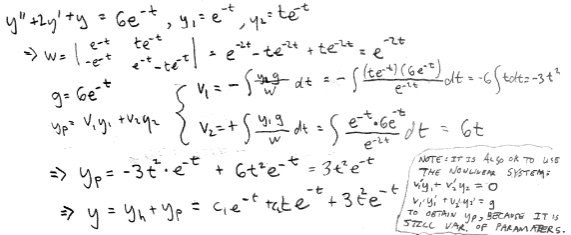
\includegraphics[width=16cm]{Images/ImgTest2VoP.jpg}
    \end{figure}  
} 
\else 
\vspace{3cm}
\fi
\fi


\ifnum \Version=2
\question[6] Consider the differential equation

    $$y'' + p(t)y' + q(t)y = 60t^3, \quad y=y(t)$$    
    
    Solutions to the corresponding homogeneous problem are $y_1 = 1$ and $y_2 = t^2$. 

    \begin{parts}
        \part Determine a particular solution to the differential equation using variation of parameters. Do not use the method of undetermined coefficients. 
        \ifnum \Solutions=0 
        \vspace{16cm}
        \fi
        \part State the general solution to the differential equation.
    \end{parts}
    \ifnum \Solutions=1 {\color{DarkBlue} 
    \begin{enumerate}
    \item[a)] The Wronskian is
\begin{align}
    W = \det \begin{pmatrix} 1&t^2\\0&2t\end{pmatrix} = 2t
\end{align}
To apply the formulas for the variation of parameters method for a second order DE we also use
\begin{align}
    y_1 & = 1 \\
    y_2 &= t^2 \\
    g &= 60t^3 
\end{align}
Applying the formulas for $v_1$ and $v_2$ we obtain
\begin{align}
    v_1 &= - \int \frac{y_2(t)g(t)}{W[y_1,y_2]}dt = - \int \frac{t^2 \cdot 60t^3}{2t} dt = - \int 30 t^4 \, dt = -6t^5 + k_1\\
    v_2 &= \int \frac{y_1(t)g(t)}{W[y_1,y_2]} dt = \int \frac{1\cdot60t^3}{2t} dt = \int 30 t^2 \, dt = 10t^3 + k_2
\end{align}
The arbitrary constants of integration, $k_1$ and $k_2$, in the above are actually not necessary. In the end they will only produce redundant terms because they are solutions to the homogeneous equation. But it is OK to leave them in the expressions for $v_1$ and $v_2$, in the expression for $y_p$, and the expression for $y$. The expression for $y_p$ becomes
\begin{align}
    y_p &= v_1y_1 + v_2y_2 \\
    &= (-6t^5 + k_1)\cdot 1 + (10t^3 + k_2) t^2 \\
    &= -6t^5 + k_1 + 10t^5 + k_2 t^2 \\
    &= 4t^5 + k_1 + k_2t^2
\end{align}
It is OK to ignore the terms with the integration constants and leave the solution as
\begin{align}
    y_p = v_1y_1 + v_2y_2 = -6t^5  + 10t^5 = 4t^5
\end{align}
\item [b)] The general solution to the differential equation is
\begin{align}
    y &= y_h + y_p \\
    &= c_1y_1 + c_2y_2 + v_1y_1 + v_2y_2 \\
    &= c_1 +c_2t^2 + 4t^5 + k_1  + k_2 t^2
\end{align}
Or we can write
\begin{align}
    y &= y_h + y_p  = c_1 +c_2t^2 + 4t^5 
\end{align}
\end{enumerate}
    } 
    \else 
    \fi    
\fi

\ifnum \Version=3
\question[6] Consider the differential equation

    $$y'' + p(t)y' + q(t)y = 60e^{-4t}, \quad y=y(t)$$    
    
    Solutions to the corresponding homogeneous problem are $y_1 = e^t$ and $y_2 = 1$. 
    
    \begin{parts}
        \part Determine a particular solution to the differential equation using variation of parameters. Do not use the method of undetermined coefficients. 
        \ifnum \Solutions=0 
        \vspace{16cm}
        \fi
        \part State the general solution to the differential equation.
    \end{parts}
    \ifnum \Solutions=1 {\color{DarkBlue}  
    \begin{enumerate}
    \item[a)] The Wronskian is
\begin{align}
    W = \det \begin{pmatrix} e^t&1\\e^t&0\end{pmatrix} = -e^t
\end{align}
The formulas for the variation of parameters method for a second order DE also uses:
\begin{align}
    y_1 & = e^t \\
    y_2 &= 1 \\
    g &= 60e^{-4t} 
\end{align}
Applying the formulas for $v_1$ and $v_2$ we obtain
\begin{align}
    v_1 &= - \int \frac{y_2(t)g(t)}{W[y_1,y_2]}dt 
    = - \int \frac{1 \cdot 60e^{-4t}}{-e^t} dt 
    = \int 60e^{-5t} \, dt 
    = -12e^{-5t} + k_1\\
    v_2 &= \int \frac{y_1(t)g(t)}{W[y_1,y_2]} dt 
    = \int \frac{e^t\cdot60e^{-4t}}{-e^t} dt 
    = - \int 60 e^{-4t}\, dt 
    = 15e^{-4t} + k_2
\end{align}
The arbitrary constants of integration, $k_1$ and $k_2$, in the above are actually not necessary. In the end they will only produce redundant terms because they are solutions to the homogeneous equation. But it is OK to leave them in the expressions for $v_1$ and $v_2$, in the expression for $y_p$, and the expression for $y$. 

The expression for $y_p$ becomes
\begin{align}
    y_p &= v_1y_1 + v_2y_2 \\
    &= (-12e^{-5t} + k_1)\cdot e^t + (15e^{-4t} + k_2) \cdot 1 \\
    &= 3e^{-4t} + k_1e^t + k_2
\end{align}
It is OK to ignore the terms with the integration constants and leave the solution as
\begin{align}
    y_p = v_1y_1 + v_2y_2 = 3e^{-4t}
\end{align}
\item [b)] The general solution to the differential equation is
\begin{align}
    y &= y_h + y_p \\
    &= c_1y_1 + c_2y_2 + v_1y_1 + v_2y_2 \\
    &= c_1e^t +c_2 + 3e^{-4t} + k_1e^t + k_2
\end{align}
Or we can write
\begin{align}
    y &= y_h + y_p  = c_1e^t +c_2 + 3e^{-4t} 
\end{align}
\end{enumerate}
    } 
    \else 
    \fi        
\fi


\ifnum \Version=4
\question[6] Consider the differential equation

    $$y'' + p(t)y' + q(t)y = 60t^3, \quad y=y(t)$$    
    
    Solutions to the corresponding homogeneous problem are $y_1 = 1$ and $y_2 = t^2$. 
    
    \begin{parts}
        \part Determine a particular solution to the differential equation using variation of parameters. Do not use the method of undetermined coefficients. 
        \ifnum \Solutions=0 
        \vspace{16cm}
        \fi
        \part State the general solution to the differential equation.
    \end{parts}
    \ifnum \Solutions=1 {\color{DarkBlue}  
    \begin{enumerate}
    \item[a)] The Wronskian is
\begin{align}
    W = \det \begin{pmatrix} 1&t^2\\0&2t\end{pmatrix} = 2t
\end{align}
To apply the formulas for the variation of parameters method for a second order DE we also use
\begin{align}
    y_1 & = 1 \\
    y_2 &= t^2 \\
    g &= 60t^3 
\end{align}
Applying the formulas for $v_1$ and $v_2$ we obtain
\begin{align}
    v_1 &= - \int \frac{y_2(t)g(t)}{W[y_1,y_2]}dt = - \int \frac{t^2 \cdot 60t^3}{2t} dt = - \int 30 t^4 \, dt = -6t^5 + k_1\\
    v_2 &= \int \frac{y_1(t)g(t)}{W[y_1,y_2]} dt = \int \frac{1\cdot60t^3}{2t} dt = \int 30 t^2 \, dt = 10t^3 + k_2
\end{align}
The arbitrary constants of integration, $k_1$ and $k_2$, in the above are actually not necessary. In the end they will only produce redundant terms because they are solutions to the homogeneous equation. But it is OK to leave them in the expressions for $v_1$ and $v_2$, in the expression for $y_p$, and the expression for $y$. The expression for $y_p$ becomes
\begin{align}
    y_p &= v_1y_1 + v_2y_2 \\
    &= (-6t^5 + k_1)\cdot 1 + (10t^3 + k_2) t^2 \\
    &= -6t^5 + k_1 + 10t^5 + k_2 t^2 \\
    &= 4t^5 + k_1 + k_2t^2
\end{align}
It is OK to ignore the terms with the integration constants and leave the solution as
\begin{align}
    y_p = v_1y_1 + v_2y_2 = -6t^5  + 10t^5 = 4t^5
\end{align}
\item [b)] The general solution to the differential equation is
\begin{align}
    y &= y_h + y_p \\
    &= c_1y_1 + c_2y_2 + v_1y_1 + v_2y_2 \\
    &= c_1 +c_2t^2 + 4t^5 + k_1  + k_2 t^2
\end{align}
Or we can write
\begin{align}
    y &= y_h + y_p  = c_1 +c_2t^2 + 4t^5 
\end{align}
\end{enumerate}
    } 
    \else 
    \fi
\fi

\ifnum \Version=5
\question[6] Consider the differential equation

    $$y'' + p(t)y' + q(t)y = 60e^{-4t}, \quad y=y(t)$$    
    
    Solutions to the corresponding homogeneous problem are $y_1 = e^t$ and $y_2 = 1$. 

    \begin{parts}
        \part Determine a particular solution to the differential equation using variation of parameters. Do not use the method of undetermined coefficients. 
        \ifnum \Solutions=0 
        \vspace{16cm}
        \fi
        \part State the general solution to the differential equation.
    \end{parts}
    \ifnum \Solutions=1 {\color{DarkBlue}  
    \begin{enumerate}
    \item[a)] The Wronskian is
\begin{align}
    W = \det \begin{pmatrix} e^t&1\\e^t&0\end{pmatrix} = -e^t
\end{align}
The formulas for the variation of parameters method for a second order DE also uses:
\begin{align}
    y_1 & = e^t \\
    y_2 &= 1 \\
    g &= 60e^{-4t} 
\end{align}
Applying the formulas for $v_1$ and $v_2$ we obtain
\begin{align}
    v_1 &= - \int \frac{y_2(t)g(t)}{W[y_1,y_2]}dt 
    = - \int \frac{1 \cdot 60e^{-4t}}{-e^t} dt 
    = \int 60e^{-5t} \, dt 
    = -12e^{-5t} + k_1\\
    v_2 &= \int \frac{y_1(t)g(t)}{W[y_1,y_2]} dt 
    = \int \frac{e^t\cdot60e^{-4t}}{-e^t} dt 
    = - \int 60 e^{-4t}\, dt 
    = 15e^{-4t} + k_2
\end{align}
The arbitrary constants of integration, $k_1$ and $k_2$, in the above are actually not necessary. In the end they will only produce redundant terms because they are solutions to the homogeneous equation. But it is OK to leave them in the expressions for $v_1$ and $v_2$, in the expression for $y_p$, and the expression for $y$. 

The expression for $y_p$ becomes
\begin{align}
    y_p &= v_1y_1 + v_2y_2 \\
    &= (-12e^{-5t} + k_1)\cdot e^t + (15e^{-4t} + k_2) \cdot 1 \\
    &= 3e^{-4t} + k_1e^t + k_2
\end{align}
It is OK to ignore the terms with the integration constants and leave the solution as
\begin{align}
    y_p = v_1y_1 + v_2y_2 = 3e^{-4t}
\end{align}
\item [b)] The general solution to the differential equation is
\begin{align}
    y &= y_h + y_p \\
    &= c_1y_1 + c_2y_2 + v_1y_1 + v_2y_2 \\
    &= c_1e^t +c_2 + 3e^{-4t} + k_1e^t + k_2
\end{align}
Or we can write
\begin{align}
    y &= y_h + y_p  = c_1e^t +c_2 + 3e^{-4t} 
\end{align}
\end{enumerate}
    } 
    \else 
    \fi    
\fi



\ifnum \Version>5
\question[4] Consider the first order system \[\vec{x} \, ' = \left( \begin{array}{rr} 2 & 4 \\ 4 & 2 \end{array} \right) \vec{x}  + \begin{pmatrix} 24\\0\end{pmatrix}  \]
    
    Solutions to the corresponding homogeneous problem are $\vec x_1 = e^{-2t}\begin{pmatrix} 1\\-1\end{pmatrix}$ and $\vec x_2 = e^{6t}\begin{pmatrix} 1\\1\end{pmatrix}$. 

    \begin{parts}
        \part Determine a particular solution to the differential equation using variation of parameters. Do not use the method of undetermined coefficients. 
\ifnum \Solutions=0 \vspace{17cm}\fi
        \part State the general solution to the system of differential equations. 
    \end{parts}
    \ifnum \Solutions=1 {\color{DarkBlue}   
    
    \begin{itemize}
        \item \textbf{Fundamental Matrix}\\
        The fundamental matrix \(X(t)\) is constructed by placing the solutions \(\vec{x}_1\) and \(\vec{x}_2\) as columns in a matrix. Thus,
        
        \[
        X(t) = \begin{pmatrix} \vec{x}_1 & \vec{x}_2 \end{pmatrix} = \begin{pmatrix} e^{-2t} & e^{6t} \\ -e^{-2t} & e^{6t} \end{pmatrix}
        \]
        \item \textbf{Inverse}\\
        \begin{align*}
            \det(X(t)) &= e^{-2t} \cdot e^{6t} - e^{6t} \cdot (-e^{-2t}) = e^{4t} + e^{4t} = 2e^{4t}\\
            X^{-1} &= \frac{1}{2e^{4t}} \begin{pmatrix} e^{6t} & -e^{6t} \\ e^{-2t} & e^{-2t} \end{pmatrix}
        = \frac{1}{2} \begin{pmatrix} e^{2t} & -e^{2t} \\ e^{-6t} & e^{-6t} \end{pmatrix}
        \end{align*}
        
        \item \textbf{Particular}\\
        \begin{align}
            \vec x_p &= X \int X^{-1} g \, dt \\
            &= X \int \frac{1}{2} \begin{pmatrix} e^{2t} & -e^{2t} \\ e^{-6t} & e^{-6t} \end{pmatrix} \begin{pmatrix} 24 \\ 0 \end{pmatrix} \, dt \\
            & = X \int \begin{pmatrix} 12e^{2t} \\ 12e^{-6t} \end{pmatrix} \, dt \\
            &= \begin{pmatrix} e^{-2t} & e^{6t} \\ -e^{-2t} & e^{6t} \end{pmatrix} \begin{pmatrix} 6e^{2t} + C_1 \\ -2e^{-6t} + C_2 \end{pmatrix} \\
            &=  \begin{pmatrix} 4 + C_1 e^{-2t} + C_2 e^{6t} \\ -8 - C_1 e^{-2t} + C_2 e^{6t} \end{pmatrix}
        \end{align}  
        It is not necessary to keep the $C_1$ and $C_2$ terms, they can be ignored. 
        \item \textbf{General Solution}
        \begin{align}
            \vec x = \vec x_h + \vec x_p = c_1 e^{-2t}\begin{pmatrix} 1\\-1\end{pmatrix} + c_2 e^{6t}\begin{pmatrix} 1\\1\end{pmatrix} + \begin{pmatrix} 4\\-8\end{pmatrix}
        \end{align}

    \end{itemize}




    } 
    \else 
    \fi    
\fi

        
        \ifnum \Version=1    
\question[2] You do not need to show your work for this question. Fill in the appropriate circle to indicate whether the following functions are exponential order. 
\vspace{-0.2cm}
\setlength{\extrarowheight}{0.10cm}
\begin{center}
\hspace{-.9cm}\begin{tabular}{ p{0.20cm} p{4cm} p{3.5cm} p{4cm} }
    & & exponential order &  not exponential order  \\[2pt] \hline 
    a) & $f(t) = t^3+1$ & $\bigcirc$  & $\bigcirc$ \\[4pt]  
    b) & $f(t) = e^{-t^2}$  & $\bigcirc$  & $\bigcirc$ \\[4pt] 
    c) & $f(t) = e^{2t^4}$  & $\bigcirc$  & $\bigcirc$ \\[4pt] 
    d) & $f(t) = \sin(3t)$  & $\bigcirc$  & $\bigcirc$ \\[4pt] 
    e) & $f(t) = 4$  & $\bigcirc$  & $\bigcirc$ \\[4pt] 
    \hline
\end{tabular}
\end{center}
\setlength{\extrarowheight}{0.0cm}
\ifnum \Solutions=1 {\color{DarkBlue} A function 
$f$ is \textbf{of exponential order} if there exists constants $K, \ a, \ M$ such that $$  |f(t)| \leq Ke^{at}  $$ for all $t > M$. In other words, $$ \frac{f(t)}{e^{at}}  $$ is bounded for sufficiently large $t$.
\begin{enumerate}[label=(\alph*)]
    \item exponential order, because $|t^3+1| < Ke^{at}$ for $K=a=1$ and $t$ greater than some value $M$. In other words, $$\lim_{t\to \infty}\frac{f(t)}{e^t} = \lim_{t\to \infty}\frac{t^3+1}{e^t} \to 0$$ We can see this by using l'Hospital's rule. 
    \item exponential order, because $$\lim_{t\to \infty}\frac{f(t)}{e^t} = \lim_{t\to \infty}\frac{e^{-t^2}}{e^t} \to 0$$
    \item not exponential order, because 
    $$\lim_{t\to \infty}\frac{f(t)}{e^t} = \lim_{t\to \infty}\frac{e^{2t^4}}{e^t} \to \infty$$ In other words, there are no values of $K,a,M$ so that $$  |f(t)| \leq Ke^{at}  $$ for all $t > M$.
    \item exponential order because $$\lim_{t\to \infty}\frac{f(t)}{e^t} = \lim_{t\to \infty}\frac{4}{e^t} \to 0$$
\end{enumerate}
}
\fi
\vspace{-6pt} 
\fi 



\ifnum \Version=2  
\question[2] You do not need to show your work for this question. Fill in the appropriate circle to indicate whether the following functions are exponential order. 
\vspace{-0.2cm}
\setlength{\extrarowheight}{0.10cm}
\begin{center}
\hspace{-.9cm}\begin{tabular}{ p{0.20cm} p{4cm} p{3.5cm} p{4cm} }
    & & exponential order &  not exponential order  \\[2pt] \hline 
    a) & $f(t) = 4$ & $\bigcirc$  & $\bigcirc$ \\[4pt]  
    b) & $f(t) = e^{t^2}$  & $\bigcirc$  & $\bigcirc$ \\[4pt] 
    c) & $f(t) = \frac{1}{(t-3)^2}$  & $\bigcirc$  & $\bigcirc$ \\[4pt]    
    d) & $f(t) = 2^t$  & $\bigcirc$  & $\bigcirc$ \\[4pt] 
    \hline
\end{tabular}
\end{center}
\setlength{\extrarowheight}{0.0cm}
\ifnum \Solutions=1 {\color{DarkBlue} A function 
$f$ is \textbf{of exponential order} if there exists constants $K, \ a, \ M$ such that $$  |f(t)| \leq Ke^{at}  $$ for all $t > M$. In other words, $$ \frac{f(t)}{e^{at}}  $$ is bounded for sufficiently large $t$.
\begin{enumerate}[label=(\alph*)]
    \item exponential order, because $|4| = 4 < Ke^{at}$ for $K=a=1$ and $t$ greater than some value $M$. In other words, $$\lim_{t\to \infty}\frac{f(t)}{e^t} = \lim_{t\to \infty}\frac{4}{e^t} \to 0$$ We can see this by using l'Hospital's rule. 
    \item not exponential order, because 
    $$\lim_{t\to \infty}\frac{f(t)}{e^t} = \lim_{t\to \infty}\frac{e^{2t^4}}{e^t} \to \infty$$ In other words, there are no values of $K,a,M$ so that $$  |f(t)| \leq Ke^{at}  $$ for all $t > M$.
    \item exponential order, because $$\lim_{t\to \infty}\frac{f(t)}{e^t} = \lim_{t\to \infty}\frac{1/((t-3)^2)}{e^t} \to 0$$    
    \item exponential order because $$\lim_{t\to \infty}\frac{f(t)}{e^t} = \lim_{t\to \infty}\frac{4}{e^t} \to 0$$
\end{enumerate}
}
\fi
\vspace{-6pt} 
\fi 


\ifnum \Version=3
\question[2] You do not need to show your work for this question. Fill in the appropriate circle to indicate whether the following functions are exponential order. 
\vspace{-0.2cm}
\setlength{\extrarowheight}{0.10cm}
\begin{center}
\hspace{-.9cm}\begin{tabular}{ p{0.20cm} p{4cm} p{3.5cm} p{4cm} }
    & & exponential order &  not exponential order  \\[2pt] \hline 
    a) & $f(t) = 1$ & $\bigcirc$  & $\bigcirc$ \\[4pt]  
    b) & $f(t) = \frac{1}{\sqrt t}$  & $\bigcirc$  & $\bigcirc$ \\[4pt] 
    c) & $f(t) = t^2$  & $\bigcirc$  & $\bigcirc$ \\[4pt] 
    d) & $f(t) = e^{-t^2}$  & $\bigcirc$  & $\bigcirc$ \\[4pt] 
    \hline
\end{tabular}
\end{center}
\setlength{\extrarowheight}{0.0cm}
\ifnum \Solutions=1 {\color{DarkBlue} A function 
$f$ is \textbf{of exponential order} if there exists constants $K, \ a, \ M$ such that $$  |f(t)| \leq Ke^{at}  $$ for all $t > M$. In other words, $$ \frac{f(t)}{e^{at}}  $$ is bounded for sufficiently large $t$.
\begin{enumerate}[label=(\alph*)]
    \item exponential order, because $|4| = 4 < Ke^{at}$ for $K=a=1$ and $t$ greater than some value $M$. In other words, $$\lim_{t\to \infty}\frac{f(t)}{e^t} = \lim_{t\to \infty}\frac{4}{e^t} \to 0$$ We can see this by using l'Hospital's rule. 
    \item not exponential order, because 
    $$\lim_{t\to \infty}\frac{f(t)}{e^t} = \lim_{t\to \infty}\frac{e^{2t^4}}{e^t} \to \infty$$ In other words, there are no values of $K,a,M$ so that $$  |f(t)| \leq Ke^{at}  $$ for all $t > M$.
    \item exponential order, because $$\lim_{t\to \infty}\frac{f(t)}{e^t} = \lim_{t\to \infty}\frac{1/((t-3)^2)}{e^t} \to 0$$    
    \item exponential order because $$\lim_{t\to \infty}\frac{f(t)}{e^t} = \lim_{t\to \infty}\frac{4}{e^t} \to 0$$
\end{enumerate}
}
\fi
\vspace{-6pt} 
\fi 




\ifnum \Version=4
\question[2] You do not need to show your work for this question. Fill in the appropriate circle to indicate whether the following functions are exponential order. 
\vspace{-0.2cm}
\setlength{\extrarowheight}{0.10cm}
\begin{center}
\hspace{-.9cm}\begin{tabular}{ p{0.20cm} p{4cm} p{3.5cm} p{4cm} }
    & & exponential order &  not exponential order  \\[2pt] \hline 
    a) & $f(t) = 4$ & $\bigcirc$  & $\bigcirc$ \\[4pt]  
    b) & $f(t) = e^{t^2}$  & $\bigcirc$  & $\bigcirc$ \\[4pt] 
    c) & $f(t) = \frac{1}{(t-3)^2}$  & $\bigcirc$  & $\bigcirc$ \\[4pt]  
    d) & $f(t) = 2^t$  & $\bigcirc$  & $\bigcirc$ \\[4pt] 
    \hline
\end{tabular}
\end{center}
\setlength{\extrarowheight}{0.0cm}
\ifnum \Solutions=1 {\color{DarkBlue} A function 
$f$ is \textbf{of exponential order} if there exists constants $K, \ a, \ M$ such that $$  |f(t)| \leq Ke^{at}  $$ for all $t > M$. In other words, $$ \frac{f(t)}{e^{at}}  $$ is bounded for sufficiently large $t$.
\begin{enumerate}[label=(\alph*)]
    \item exponential order, because $|4| = 4 < Ke^{at}$ for $K=a=1$ and $t$ greater than some value $M$. In other words, $$\lim_{t\to \infty}\frac{f(t)}{e^t} = \lim_{t\to \infty}\frac{4}{e^t} \to 0$$ We can see this by using l'Hospital's rule. 
    \item not exponential order, because 
    $$\lim_{t\to \infty}\frac{f(t)}{e^t} = \lim_{t\to \infty}\frac{e^{2t^4}}{e^t} \to \infty$$ In other words, there are no values of $K,a,M$ so that $$  |f(t)| \leq Ke^{at}  $$ for all $t > M$.
    \item exponential order, because $$\lim_{t\to \infty}\frac{f(t)}{e^t} = \lim_{t\to \infty}\frac{1/((t-3)^2)}{e^t} \to 0$$    
    \item exponential order because $$\lim_{t\to \infty}\frac{f(t)}{e^t} = \lim_{t\to \infty}\frac{4}{e^t} \to 0$$
\end{enumerate}
}
\fi
\vspace{-6pt} 
\fi 


\ifnum \Version=5
\question[2] You do not need to show your work for this question. Fill in the appropriate circle to indicate whether the following functions are exponential order. 
\vspace{-0.2cm}
\setlength{\extrarowheight}{0.10cm}
\begin{center}
\hspace{-.9cm}\begin{tabular}{ p{0.20cm} p{4cm} p{3.5cm} p{4cm} }
    & & exponential order &  not exponential order  \\[2pt] \hline 
    a) & $f(t) = 1$ & $\bigcirc$  & $\bigcirc$ \\[4pt]  
    b) & $f(t) = \frac{1}{\sqrt t}$  & $\bigcirc$  & $\bigcirc$ \\[4pt]  
    c) & $f(t) = t^2$  & $\bigcirc$  & $\bigcirc$ \\[4pt] 
    d) & $f(t) = e^{-t^2}$  & $\bigcirc$  & $\bigcirc$ \\[4pt] 
    \hline
\end{tabular}
\end{center}
\setlength{\extrarowheight}{0.0cm}
\ifnum \Solutions=1 {\color{DarkBlue} A function 
$f$ is \textbf{of exponential order} if there exists constants $K, \ a, \ M$ such that $$  |f(t)| \leq Ke^{at}  $$ for all $t > M$. In other words, $$ \frac{f(t)}{e^{at}}  $$ is bounded for sufficiently large $t$.
\begin{enumerate}[label=(\alph*)]
    \item exponential order, because $|4| = 4 < Ke^{at}$ for $K=a=1$ and $t$ greater than some value $M$. In other words, $$\lim_{t\to \infty}\frac{f(t)}{e^t} = \lim_{t\to \infty}\frac{4}{e^t} \to 0$$ We can see this by using l'Hospital's rule. 
    \item not exponential order, because 
    $$\lim_{t\to \infty}\frac{f(t)}{e^t} = \lim_{t\to \infty}\frac{e^{2t^4}}{e^t} \to \infty$$ In other words, there are no values of $K,a,M$ so that $$  |f(t)| \leq Ke^{at}  $$ for all $t > M$.
    \item exponential order, because $$\lim_{t\to \infty}\frac{f(t)}{e^t} = \lim_{t\to \infty}\frac{1/((t-3)^2)}{e^t} \to 0$$    
    \item exponential order because $$\lim_{t\to \infty}\frac{f(t)}{e^t} = \lim_{t\to \infty}\frac{4}{e^t} \to 0$$
\end{enumerate}
}
\fi
\vspace{-6pt} 
\fi 




\ifnum \Version=6
\question[2] You do not need to show your work for this question. Fill in the appropriate circle to indicate whether the following functions are exponential order. 
\vspace{-0.2cm}
\setlength{\extrarowheight}{0.10cm}
\begin{center}
\hspace{-.9cm}\begin{tabular}{ p{0.20cm} p{4cm} p{3.5cm} p{4cm} }
    & & exponential order &  not exponential order  \\[6pt] \hline 
    a) & $\displaystyle f(t) = e^{\sqrt t}$  & $\bigcirc$  & $\bigcirc$ \\[4pt] 
    b) & $f(t) = e^{t^2/4}$  & $\bigcirc$  & $\bigcirc$ \\[4pt] 
    c) & $f(t) = \sqrt{t}$ & $\bigcirc$  & $\bigcirc$ \\[4pt]  
    d) & $f(t) = 1+\ln t$  & $\bigcirc$  & $\bigcirc$ \\[4pt]  

    \hline
\end{tabular}
\end{center}
\setlength{\extrarowheight}{0.0cm}
\ifnum \Solutions=1 {\color{DarkBlue} A function 
$f$ is \textbf{exponential order} (EO) if there exists constants $K, \ a, \ M$ such that $$  |f(t)| \leq Ke^{at}  $$ for all $t > M$. In other words, $f$ is EO $$ \frac{f(t)}{e^{at}}  $$ is bounded for sufficiently large $t$.
\begin{enumerate}[label=(\alph*)]
    \item EO because $f < Ke^{at}$ for $K=a=1$ and $t > M=1$. 
    \item Not EO because 
    $$\lim_{t\to \infty}\frac{f(t)}{e^{t}} = \lim_{t\to \infty}\frac{e^{t^2/4}}{e^t} \to \infty$$ In other words, there are no values of $K,a,M$ so that $$  |f(t)| \leq Ke^{at}  $$ for all $t > M$.
    \item exponential order, because $$\lim_{t\to \infty}\frac{f(t)}{e^t} = \lim_{t\to \infty}\frac{\sqrt t}{e^t} \to 0$$    
    \item exponential order because $$\lim_{t\to \infty}\frac{f(t)}{e^t} = \lim_{t\to \infty}\frac{1+\ln t}{e^t} \to 0$$
\end{enumerate}
}
\fi
\vspace{-6pt} 
\fi 



\ifnum \Version=7
\question[2] You do not need to show your work for this question. Fill in the appropriate circle to indicate whether the following functions are exponential order. 
\vspace{-0.2cm}
\setlength{\extrarowheight}{0.10cm}
\begin{center}
\hspace{-.9cm}\begin{tabular}{ p{0.20cm} p{4cm} p{3.5cm} p{4cm} }
    & & exponential order &  not exponential order  \\[4pt] \hline 
    a) & $f(t) = e^{t^2-t}$  & $\bigcirc$  & $\bigcirc$ \\[4pt] 
    b) & $f(t) = e^{\sqrt t}$  & $\bigcirc$  & $\bigcirc$ \\[4pt] 
    c) & $f(t) = |t|+\sin t$ & $\bigcirc$  & $\bigcirc$ \\[4pt]  
    d) & $\displaystyle f(t) = \frac{t^2+3}{t+4}$  & $\bigcirc$  & $\bigcirc$ \\[6pt]  

    \hline
\end{tabular}
\end{center}
\setlength{\extrarowheight}{0.0cm}
\ifnum \Solutions=1 {\color{DarkBlue} A function 
$f$ is \textbf{of exponential order} (EO) if there exists constants $K, \ a, \ M$ such that $$  |f(t)| \leq Ke^{at}  $$ for all $t > M$. In other words, $f$ is EO $$ \frac{f(t)}{e^{at}}  $$ is bounded for sufficiently large $t$.
\begin{enumerate}[label=(\alph*)]
    \item Not EO because 
    $$\lim_{t\to \infty}\frac{f(t)}{e^t} = \lim_{t\to \infty}\frac{e^{2t^4}}{e^t} \to \infty$$ In other words, there are no values of $K,a,M$ so that $$  |f(t)| \leq Ke^{at}  $$ for all $t > M$.
    \item EO because $f < Ke^{at}$ for $K=a=1$ and $t > M=1$. 
    \item EO because $$\lim_{t\to \infty}\frac{f(t)}{e^t} = \lim_{t\to \infty}\frac{|t| + \sin t}{e^t} \to 0$$    
    \item EO because $e^t$ goes to infinity faster than $f$. 
\end{enumerate}
}
\fi
\vspace{-6pt} 
\fi 

        \ifnum \Version=1
\question[2] Determine the values of $r$ so that the differential equation $\displaystyle t^2y'' -4ty' +6y =0$ will have solutions of the form $\displaystyle y = t^r$ for $t>0$. Please show your work.
\ifnum \Solutions=1 {\color{DarkGreen} \\[12pt] 
\textbf{Solutions:} substitute $y=t^r$ into the equation to obtain:
\begin{align}
    0 &= t^2y'' -4ty' +6y \\
    &= t^2(t^r)'' - 4t(t^r)' + 6(t^r) \\ 
    &= t^2r(r-1)(t^{r-2}) - 4tr(t^{r-1}) + 6(t^r) \\ 
    &= r(r-1)(t^{r}) - 4r(t^{r}) + 6(t^r) \\ 
    &= r(r-1) - 4r + 6 \\ 
    &= r^2 - 5r + 6 \\ 
    &= (r-2)(r-3) 
\end{align}
Therefore $r=2,3$. 
} 
\else 
\fi\fi 

\ifnum \Version=6
\SecondOrderConstCo{5}{6}
\fi


\ifnum \Version=7
\SecondOrderCauchyEuler{2}{1}
\fi

\ifnum \Version=8
\SecondOrderConstCo{4}{8}
\fi


\ifnum \Version=9
\SecondOrderCauchyEuler{1}{3}
\fi


        \ifnum \Version=1

\question[2] A spring is hung from a horizontal surface as in the figure below. A mass of $m=0.2$ kg stretches the spring 0.04 m. Frictional forces also exert a force on the mass while it is moving that is proportional to the velocity of the mass. The proportionality constant for these frictional forces is 2 N s/m. The mass is then pulled down an additional 0.03 m and then released from rest. Assume that position of the mass, $y$, increases as the mass moves down. Write down an IVP based on this physical description that describes the position of the mass $y(t)$, as a function of time, $t$. You do not need to solve your IVP. \\[4pt]
\input{2023Summer/Quiz4/DiagramSpringMass}
\vspace{2cm}
\fi 


\ifnum \Version=2
\question[2] A small car with mass $m = 0.2$ kg is moving along a straight line on a horizontal surface. The car is attached to a spring. The spring exerts a force of $4$ N when it is extended a distance of $0.8$ meters from its equilibrium position. Frictional forces also exert a force on the car while it is moving that is proportional to the velocity of the car. The proportionality constant for these frictional forces is $0.6$ N s/m. The car also has an engine that pushes the car forward with a force of $F = 0.5t$ N. The car is released from rest after it is moved 0.01 m to the right of its equilibrium position. Assume that position of the car, $y$, increases as the car move to the right. Write down the IVP based on this physical description that describes the position of the car as a function of time, $t$. You do not need to solve your IVP. \\
\hspace{1cm}\begin{tikzpicture}
\tikzstyle{spring}=[thick,decorate,decoration={zigzag,pre length=0.3cm,post length=0.3cm,segment length=6}]
\tikzstyle{damper}=[thick,decoration={markings,  
  mark connection node=dmp,
  mark=at position 0.5 with 
  {
    \node (dmp) [thick,inner sep=0pt,transform shape,rotate=-90,minimum width=15pt,minimum height=3pt,draw=none] {};
    \draw [thick] ($(dmp.north east)+(2pt,0)$) -- (dmp.south east) -- (dmp.south west) -- ($(dmp.north west)+(2pt,0)$);
    \draw [thick] ($(dmp.north)+(0,-5pt)$) -- ($(dmp.north)+(0,5pt)$);
  }
}, decorate]

% WALL PATTERN
\tikzstyle{ground}=[fill,pattern=north east lines,draw=none,minimum width=0.5cm,minimum height=0.3cm,inner sep=0pt,outer sep=0pt]

% CART
\node [style={draw,outer sep=0pt,very thick}] (M) [minimum width=1cm, minimum height=1.0cm] {$m$};
% WHEELS
\draw [very thick] (M.south west) ++ (0.2cm,-0.125cm) circle (0.125cm)  (M.south east) ++ (-0.2cm,-0.125cm) circle (0.125cm);

% BOTTOM GROUND
\node (ground) [ground,anchor=north,yshift=-0.25cm,minimum width=5.6cm,xshift=-0.03cm] at (M.south) {};
\draw (ground.north east) -- (ground.north west);
\draw (ground.south east) -- (ground.south west);
\draw (ground.north east) -- (ground.south east);

% WEST WALL
\node (wall) [ground, rotate=-90, minimum width=3cm,xshift=-0.42cm,yshift=-3cm] {};
\draw (wall.north east) -- (wall.north west);
\draw (wall.north west) -- (wall.south west);
\draw (wall.south west) -- (wall.south east);
\draw (wall.south east) -- (wall.north east);

% DAMPER AND SPRING
\draw [spring] (wall.20) -- ($(M.north west)!(wall.20)!(M.south west)$);
% \node (y) at (wall.130) [yshift = 0.02cm,xshift=1.2cm] {$k$};

\end{tikzpicture}

\fi 

\ifnum \Version=3
\question[2] A small car with mass $m = 0.1$ kg is moving along a straight line on a horizontal surface. The car is attached to a spring. The spring exerts a force of $2$ N when it is extended a distance of $0.1$ meters from its equilibrium position. Frictional forces also exert a force on the car while it is moving that is proportional to the velocity of the car. The proportionality constant for these frictional forces is $0.3$ N s/m. The car also has an engine that pushes the car forward with a force of $F = 0.1$ N. The car is released from rest after it is moved 0.01 m to the left of its equilibrium position. Assume that position of the car, $y$, increases as the car move to the right. Write down the IVP based on this physical description that describes the position of the car as a function of time, $t$. You do not need to solve your IVP. \\
\hspace{1cm}\begin{tikzpicture}
\tikzstyle{spring}=[thick,decorate,decoration={zigzag,pre length=0.3cm,post length=0.3cm,segment length=6}]
\tikzstyle{damper}=[thick,decoration={markings,  
  mark connection node=dmp,
  mark=at position 0.5 with 
  {
    \node (dmp) [thick,inner sep=0pt,transform shape,rotate=-90,minimum width=15pt,minimum height=3pt,draw=none] {};
    \draw [thick] ($(dmp.north east)+(2pt,0)$) -- (dmp.south east) -- (dmp.south west) -- ($(dmp.north west)+(2pt,0)$);
    \draw [thick] ($(dmp.north)+(0,-5pt)$) -- ($(dmp.north)+(0,5pt)$);
  }
}, decorate]

% WALL PATTERN
\tikzstyle{ground}=[fill,pattern=north east lines,draw=none,minimum width=0.5cm,minimum height=0.3cm,inner sep=0pt,outer sep=0pt]

% CART
\node [style={draw,outer sep=0pt,very thick}] (M) [minimum width=1cm, minimum height=1.0cm] {$m$};
% WHEELS
\draw [very thick] (M.south west) ++ (0.2cm,-0.125cm) circle (0.125cm)  (M.south east) ++ (-0.2cm,-0.125cm) circle (0.125cm);

% BOTTOM GROUND
\node (ground) [ground,anchor=north,yshift=-0.25cm,minimum width=5.6cm,xshift=-0.03cm] at (M.south) {};
\draw (ground.north east) -- (ground.north west);
\draw (ground.south east) -- (ground.south west);
\draw (ground.north east) -- (ground.south east);

% WEST WALL
\node (wall) [ground, rotate=-90, minimum width=3cm,xshift=-0.42cm,yshift=-3cm] {};
\draw (wall.north east) -- (wall.north west);
\draw (wall.north west) -- (wall.south west);
\draw (wall.south west) -- (wall.south east);
\draw (wall.south east) -- (wall.north east);

% DAMPER AND SPRING
\draw [spring] (wall.20) -- ($(M.north west)!(wall.20)!(M.south west)$);
% \node (y) at (wall.130) [yshift = 0.02cm,xshift=1.2cm] {$k$};

\end{tikzpicture}

\fi 

\ifnum \Version=4
\question[2] A small car with mass $m = 0.2$ kg is moving along a straight line on a horizontal surface. The car is attached to a spring. The spring exerts a force of $4$ N when it is extended a distance of $0.8$ meters from its equilibrium position. Frictional forces also exert a force on the car while it is moving that is proportional to the velocity of the car. The proportionality constant for these frictional forces is $0.6$ N s/m. The car also has an engine that pushes the car forward with a force of $F = 0.5t$ N. The car is released from rest after it is moved 0.05 m to the left of its equilibrium position. Assume that position of the car, $y$, increases as the car move to the right. Write down the IVP based on this physical description that describes the position of the car as a function of time, $t$. You do not need to solve your IVP. \\
\hspace{1cm}\begin{tikzpicture}
\tikzstyle{spring}=[thick,decorate,decoration={zigzag,pre length=0.3cm,post length=0.3cm,segment length=6}]
\tikzstyle{damper}=[thick,decoration={markings,  
  mark connection node=dmp,
  mark=at position 0.5 with 
  {
    \node (dmp) [thick,inner sep=0pt,transform shape,rotate=-90,minimum width=15pt,minimum height=3pt,draw=none] {};
    \draw [thick] ($(dmp.north east)+(2pt,0)$) -- (dmp.south east) -- (dmp.south west) -- ($(dmp.north west)+(2pt,0)$);
    \draw [thick] ($(dmp.north)+(0,-5pt)$) -- ($(dmp.north)+(0,5pt)$);
  }
}, decorate]

% WALL PATTERN
\tikzstyle{ground}=[fill,pattern=north east lines,draw=none,minimum width=0.5cm,minimum height=0.3cm,inner sep=0pt,outer sep=0pt]

% CART
\node [style={draw,outer sep=0pt,very thick}] (M) [minimum width=1cm, minimum height=1.0cm] {$m$};
% WHEELS
\draw [very thick] (M.south west) ++ (0.2cm,-0.125cm) circle (0.125cm)  (M.south east) ++ (-0.2cm,-0.125cm) circle (0.125cm);

% BOTTOM GROUND
\node (ground) [ground,anchor=north,yshift=-0.25cm,minimum width=5.6cm,xshift=-0.03cm] at (M.south) {};
\draw (ground.north east) -- (ground.north west);
\draw (ground.south east) -- (ground.south west);
\draw (ground.north east) -- (ground.south east);

% WEST WALL
\node (wall) [ground, rotate=-90, minimum width=3cm,xshift=-0.42cm,yshift=-3cm] {};
\draw (wall.north east) -- (wall.north west);
\draw (wall.north west) -- (wall.south west);
\draw (wall.south west) -- (wall.south east);
\draw (wall.south east) -- (wall.north east);

% DAMPER AND SPRING
\draw [spring] (wall.20) -- ($(M.north west)!(wall.20)!(M.south west)$);
% \node (y) at (wall.130) [yshift = 0.02cm,xshift=1.2cm] {$k$};

\end{tikzpicture}

\fi 


\ifnum \Version=5
\question[2] A small car with mass $m = 0.2$ kg is moving along a straight line on a horizontal surface. The car is attached to a spring. The spring exerts a force of $8$ N when it is extended a distance of $0.2$ meters from its equilibrium position. Frictional forces also exert a force on the car while it is moving that is proportional to the velocity of the car. The proportionality constant for these frictional forces is $0.3$ N s/m. The car also has an engine that pushes the car forward with a force of $F = 2t$ N. The car is released from rest after it is moved 0.01 m to the left of its equilibrium position. Assume that position of the car, $y$, increases as the car move to the right. Write down the IVP based on this physical description that describes the position of the car as a function of time, $t$. You do not need to solve your IVP. \\
\hspace{1cm}\begin{tikzpicture}
\tikzstyle{spring}=[thick,decorate,decoration={zigzag,pre length=0.3cm,post length=0.3cm,segment length=6}]
\tikzstyle{damper}=[thick,decoration={markings,  
  mark connection node=dmp,
  mark=at position 0.5 with 
  {
    \node (dmp) [thick,inner sep=0pt,transform shape,rotate=-90,minimum width=15pt,minimum height=3pt,draw=none] {};
    \draw [thick] ($(dmp.north east)+(2pt,0)$) -- (dmp.south east) -- (dmp.south west) -- ($(dmp.north west)+(2pt,0)$);
    \draw [thick] ($(dmp.north)+(0,-5pt)$) -- ($(dmp.north)+(0,5pt)$);
  }
}, decorate]

% WALL PATTERN
\tikzstyle{ground}=[fill,pattern=north east lines,draw=none,minimum width=0.5cm,minimum height=0.3cm,inner sep=0pt,outer sep=0pt]

% CART
\node [style={draw,outer sep=0pt,very thick}] (M) [minimum width=1cm, minimum height=1.0cm] {$m$};
% WHEELS
\draw [very thick] (M.south west) ++ (0.2cm,-0.125cm) circle (0.125cm)  (M.south east) ++ (-0.2cm,-0.125cm) circle (0.125cm);

% BOTTOM GROUND
\node (ground) [ground,anchor=north,yshift=-0.25cm,minimum width=5.6cm,xshift=-0.03cm] at (M.south) {};
\draw (ground.north east) -- (ground.north west);
\draw (ground.south east) -- (ground.south west);
\draw (ground.north east) -- (ground.south east);

% WEST WALL
\node (wall) [ground, rotate=-90, minimum width=3cm,xshift=-0.42cm,yshift=-3cm] {};
\draw (wall.north east) -- (wall.north west);
\draw (wall.north west) -- (wall.south west);
\draw (wall.south west) -- (wall.south east);
\draw (wall.south east) -- (wall.north east);

% DAMPER AND SPRING
\draw [spring] (wall.20) -- ($(M.north west)!(wall.20)!(M.south west)$);
% \node (y) at (wall.130) [yshift = 0.02cm,xshift=1.2cm] {$k$};

\end{tikzpicture}

\fi 



\ifnum \Version=6

\question[6] Solve the following Cauchy-Euler equation. 
$$t^2y'' - 6ty' + 6y = 0, \quad t > 0$$

You may find the following table of formulas to be helpful. 

\begin{center}
    \begin{tabular}{ p{6.2cm} p{6cm} }
        roots &  general solution 
        \\[2pt] \hline 
        real distinct, $m_1 \ne m_2$ &  $c_1 t^{m_1} + c_2 t^{m_2}$\\       
        real repeated, $m = m_1 = m_2$ & $c_1 t^{m} + c_2 t^m \ln(t)$\\
        complex, $m_1 = \alpha + i \beta$ & $c_1t^{\alpha}\cos(\beta \ln(t)) + c_2t^{\alpha}\sin(\beta \ln (t))$\\[2pt] \hline
    \end{tabular}    
\end{center}

\ifnum \Solutions=1 {\color{DarkBlue} 
\textbf{Solutions:}

To solve the differential equation \( t^2 y'' - 6t y' + 6y = 0 \), we recognize it as a Cauchy-Euler equation. The solution to a Cauchy-Euler equation can be found by assuming a solution of the form \( y = t^r \). 

\begin{enumerate}
    \item First, we substitute \( y = t^r \) into the differential equation. We need the first and second derivatives of \( y \):
   \[ y = t^r \]
   \[ y' = r t^{r-1} \]
   \[ y'' = r (r-1) t^{r-2} \]

    \item Substitute these into the differential equation:
   \[ t^2 (r (r-1) t^{r-2}) - 6t (r t^{r-1}) + 6 t^r = 0 \]
   \[ r (r-1) t^r - 6r t^r + 6 t^r = 0 \]
   \[ (r (r-1) - 6r + 6) t^r = 0 \]
   \[ (r^2 - r - 6r + 6) t^r = 0 \]
   \[ (r^2 - 7r + 6) t^r = 0 \]

    \item Since \( t^r \neq 0 \) for \( t \neq 0 \), we set the characteristic polynomial to zero:
   \[ r^2 - 7r + 6 = 0 \]
   \[ (r - 1)(r - 6) = 0 \]
   So \( r = 1 \) and \( r = 6 \).

    \item Therefore, the general solution to the differential equation is:
   \[ y(t) = C_1 t^1 + C_2 t^6 \]
   \[ y(t) = C_1 t + C_2 t^6 \]

where \( C_1 \) and \( C_2 \) are arbitrary constants.
\end{enumerate}


} 
\else 
\newpage
\fi
\fi 


\ifnum \Version=7
\question[6] Solve the following Cauchy-Euler equation. 
$$t^2y'' - 5ty' + 5y = 0, \quad t > 0$$

You may find the following table of formulas to be helpful. 

\begin{center}
    \begin{tabular}{ p{6.2cm} p{6cm} }
        roots &  general solution 
        \\[2pt] \hline 
        real distinct, $m_1 \ne m_2$ &  $c_1 t^{m_1} + c_2 t^{m_2}$\\       
        real repeated, $m = m_1 = m_2$ & $c_1 t^{m} + c_2 t^m \ln(t)$\\
        complex, $m_1 = \alpha + i \beta$ & $c_1t^{\alpha}\cos(\beta \ln(t)) + c_2t^{\alpha}\sin(\beta \ln (t))$\\[2pt] \hline
    \end{tabular}    
\end{center}

\ifnum \Solutions=1 {\color{DarkBlue} 
\textbf{Solutions:}
To solve the differential equation \( t^2 y'' - 5t y' + 5y = 0 \), we recognize it as a Cauchy-Euler equation. The solution to a Cauchy-Euler equation can be found by assuming a solution of the form \( y = t^r \). 

\begin{enumerate}
    \item First, we substitute \( y = t^r \) into the differential equation. We need the first and second derivatives of \( y \):
   \[ y = t^r \]
   \[ y' = r t^{r-1} \]
   \[ y'' = r (r-1) t^{r-2} \]

    \item Substitute these into the differential equation and combine like terms:
   \[ t^2 (r (r-1) t^{r-2}) - 5t (r t^{r-1}) + 5 t^r = 0 \]
   \[ r (r-1) t^r - 5r t^r + 5 t^r = 0 \]
   \[ (r (r-1) - 5r + 5) t^r = 0 \]
   \[ (r^2 - r - 5r + 5) t^r = 0 \]
   \[ (r^2 - 6r + 5) t^r = 0 \]

    \item Since \( t^r \neq 0 \) for \( t \neq 0 \), we set the characteristic polynomial to zero:
   \[ r^2 - 6r + 5 = 0 \]

    \item Solve the characteristic polynomial:
   \[ r^2 - 6r + 5 = 0 \quad \Rightarrow \quad (r - 1)(r - 5) = 0 \]
   So \( r = 1 \) and \( r = 5 \).

    \item Therefore, the general solution to the differential equation is:
   \[ y(t) = C_1 t^1 + C_2 t^5 \]
   \[ y(t) = C_1 t + C_2 t^5 \]

where \( C_1 \) and \( C_2 \) are arbitrary constants.
\end{enumerate}


} 
\else 
\newpage
\fi
\fi 

        \ifnum \Version=4
            \renewcommand{\Version}{2}
        \fi
        \ifnum \Version=5
            \renewcommand{\Version}{3}
        \fi              
        \ifnum \Solutions=0
\newpage 
\fi
\ifnum \Version=1    
    \question[6] Use the Laplace transform to solve the following IVP. Do not leave your answer in terms of an integral. Please show your work.
    % $$\displaystyle y''-4y'+4y=0,\qquad y(0)=1,\quad y'(0)=1$$ %Q,A HW 5.4#4
    % $$\displaystyle y''-2y'+4y=0,\qquad y(0)=2,\quad y'(0)=0$$ %M HW 5.4#5
    $$ y'' -6y'+13y = 0, \quad y(0) = 0, \quad y'(0) = -3$$. % A TRIM P301 #27
    % $$ y''+ 2y'+y = 0, \quad y(0) = 1, \quad y'(0) = 1$$. % B TRIM P301 #23
\ifnum \Solutions=1 {\color{DarkBlue} 
Take the transform of the DE and solve for $Y(s) = \mathcal{L}[y(t)]$.
\begin{align}
    0
    &= s^2Y-sy(0) - y'(0) - 6(sY-y(0)) + 13Y \\
    &= s^2Y-0 +3 - 6(sY-0) + 13Y \\
    -3 &= s^2Y - 6sY + 13Y \\
    -3 &= (s^2 - 6s + 13)Y \\
    Y &= \frac{-3}{s^2- 6s+13} 
\end{align}    
Complete the square:
\begin{align}
    Y &= \frac{-3}{s^2- 6s+9-9+13} = \frac{-3}{ (s-3)^2+4}=\frac{-3}{2}\cdot \frac{2}{ (s-3)^2+4}
\end{align}    
Inverse transform:
\begin{align}
    y(t) &= \frac{-3}{2}\sin(2t)e^{3t}
\end{align}
} 
\else 
\vspace{3cm}
\fi
\fi 



\ifnum \Version=2
    \question[6] Consider the IVP: $y''+4y'+3y = 4e^{-2t}$, $y(0)=0, y'(0) = 0$. 
        \begin{parts}
        \part Use the Laplace Transform to obtain an explicit expression for $Y(s) = \mathcal{L}[y]$. 
        \ifnum \Solutions=1 {\color{DarkBlue} \\[12pt] 
        Taking the transform of the IVP yields
        \begin{align}
            s^2Y-sy(0) - y'(0) +4(sY-y(0)) +3 Y &= \frac{4}{s+2} \\
            (s^2 +4s+3)Y &= \frac{4}{s+2} \\
            Y&= \frac{1}{s+2} \frac{4}{s^2 +4s+3} \\
            &= \frac{4}{(s+1)(s+2)(s+3)}
        \end{align}
        } 
        \else 
        \vfill
        \fi
        \part Use the inverse Laplace Transform to solve the IVP. 
        \ifnum \Solutions=1 {\color{DarkBlue} \\[12pt] 
        Partial fractions: 
        \begin{align}
            \frac{4}{(s+2)(s+1)(s+3)} & = \frac{A}{s+1} + \frac{B}{s+2} + \frac{C}{s+3} \\
            4 & = A(s+2)(s+3) + B(s+1)(s+3) + C(s+1)(s+2) 
        \end{align}
        Selecting values of $s$ yields
        \begin{align}
            s=-1: \quad 4 & = 2A + 0 + 0 \quad \Rightarrow \quad A = 2 \\
            s=-2: \quad 4 & = 0 - B + 0 \quad \Rightarrow \quad B = -4 \\
            s=-3: \quad 4 & = 0 + 0 + 2C \quad \Rightarrow \quad C = 2
        \end{align}
        Thus
       \begin{align}
            Y (s) = \frac{4}{(s+1)(s+2)(s+3)} 
            &= \frac{A}{s+1} + \frac{B}{s+2} + \frac{C}{s+3} \\
            &= \frac{2}{s+1} + \frac{-4}{s+2} + \frac{2}{s+3} 
        \end{align}        
        With the inverse transform this becomes 
        \begin{align}
            y(t) &= 2e^{-t} -4 e^{-2t} +2 e^{-3t}
        \end{align}
        } 
        \else 
        \vfill
        \fi
    \end{parts}
\fi 




\ifnum \Version>5
    \question[4] Consider the IVP: $y''+4y = 8e^{-2t}$, $y(0)=0, y'(0) = 0$. 
        \begin{parts}
        \part Use the Laplace Transform to obtain an explicit expression for $Y(s) = \mathcal{L}[y]$. 
        \ifnum \Solutions=1 {\color{DarkBlue} \\[12pt] 
        Taking the transform of the IVP yields
        \begin{align}
            s^2Y-sy(0) - y'(0) + 4 Y &= \frac{8}{s+2} \\
            (s^2 + 4)Y &= \frac{8}{s+2} \\
            Y&= \frac{8}{s+2} \frac{1}{s^2 + 4} \\
            &= \frac{8}{(s^2+4)(s+2)}
        \end{align}
        } 
        \else 
        \vfill
        \fi
        \part Use the inverse Laplace Transform to solve the IVP. 
        \ifnum \Solutions=1 {\color{DarkBlue} \\[12pt] 
        Partial fractions: 
        \begin{align}
            \frac{8}{(s^2+4)(s+2)} & = \frac{As+B}{s^2+4} + \frac{C}{s+2} \\
            8 & = (As+B)(s+2) + C(s^2+4) \\
            8 &= (A+C)s^2 +(2A+B)s+(2B+4C)
        \end{align}
        Selecting $s = -2$ yields
        \begin{align}
            s=-2: \quad 8 & = 0 + C((-2)^2+4) \quad \Rightarrow \quad C = 1 
        \end{align}
        The quadratic terms give us 
        \begin{align}
            A+C = 0 \Rightarrow \quad A = - 1 
        \end{align}
        The linear terms give us 
        \begin{align}
            2A+B = 0 \Rightarrow \quad B = 2
        \end{align}        
        Thus
       \begin{align}
            Y (s) = \frac{8}{(s^2+4)(s+2)} 
            &= \frac{As+B}{s^2+4} + \frac{C}{s+2} \\
            &= \frac{-s+2}{s^2+4} + \frac{1}{s+2} \\
            &= -\frac{s}{s^2+4} + \frac{2}{s^2+4} + \frac{1}{s+2} \\
        \end{align}        
        With the inverse transform this becomes 
        \begin{align}
            y(t) &= \sin(2t) - \cos(2t) + e^{-2t}
        \end{align}
        \textbf{Additional Notes}\\
        Some students made an error in taking the transform that resulted in the expression
        $$Y = \frac{8}{s(s+4)(s+2)} = \frac1s+\frac{1}{s+4}- \frac{2}{s+2}$$
        } 
        \else 
        \vfill
        \fi
    \end{parts}
\fi 


        \ifnum \Solutions=0
\newpage 
\fi
\ifnum \Version=1
    \question[5] Consider the non-linear system below.  
    \begin{align*}
        \dxdt &= y(x+y-6) , \qquad \dydt = x(2x+y-8)
    \end{align*}
    \begin{parts}
        \part Determine the locations of the critical points. 
        \ifnum \Solutions=1 {\color{DarkBlue} \\[12pt] 
        Setting both $x'=0$ and $y'=0$, we obtain four critical points as follows. $x'=0$ implies $y=0$ or $x+y-6=0$. 
            \begin{itemize}
                \item If $y=0$, then for $y'=0$ we need either $x=0$ or $2x+y-8=0$. 
                \begin{itemize}
                    \item If $y=0$ and $x=0$, one critical point is at $(0,0)$. 
                    \item If $y=0$ and $2x+y-8=0$, one critical point is at $(4,0)$. 
                \end{itemize}
                \item If $x+y-6=0$, then for $y'=0$ we need either $x=0$ or $2x+y-8=0$. 
                \begin{itemize}
                    \item If $x+y-6=0$ and $x=0$, one critical point is at $(0,6)$. 
                    \item If $x+y-6=0$ and $2x+y-8=0$, then solving this system of equations yields a critical point at $(2,4)$. 
                \end{itemize}                
            \end{itemize}
            The four critical points are located at $(0,0)$, $(4,0)$, $(0,6)$, $(2,4)$. 
            } 
        \else 
        \vfill
        \fi
        \part Sketch the nullclines of the system on the axes below. Clearly indicate the critical points that you found in part (a). 
        \ifnum \Solutions=1 {\color{DarkBlue} \\[12pt] 
        Green lines are the $x-$nullclines, red lines are the $y-$nullclines.
        \begin{center}
        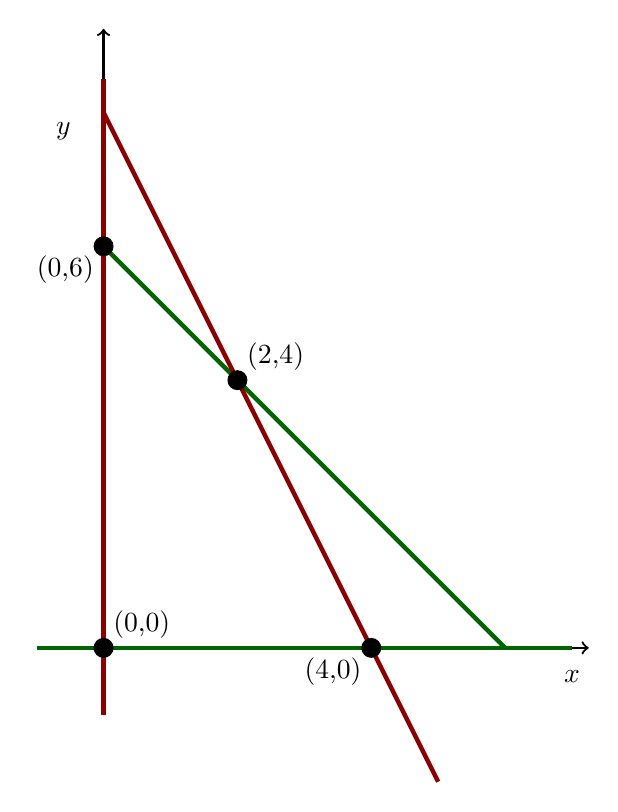
\begin{tikzpicture}[scale=0.85]
        \draw[thick, ->] (-1, 0) -- (7.25, 0);
        \draw[thick, ->] (0, -1) -- (0, 9.25);
        \node[overlay, below] at (7, -0.2) {$x$};
        \node[overlay, below] at (-0.6, 8) {$y$};   
        \draw[ultra thick,DarkGreen, -] (-1, 0) -- (7, 0);        
        \draw[ultra thick,DarkGreen, -] (0,6) -- (6, 0);   
        \draw[ultra thick,DarkRed, -] (0, 8) -- (5, -2);        
        \draw[ultra thick,DarkRed, -] (0, -1) -- (0, 8.5);      
        \filldraw[black] (0,0) circle (4pt) node[anchor=south west]{(0,0)};
        \filldraw[black] (0,6) circle (4pt) node[anchor=north east]{(0,6)};
        \filldraw[black] (2,4) circle (4pt) node[anchor=south west]{(2,4)};
        \filldraw[black] (4,0) circle (4pt) node[anchor=north east]{(4,0)};
        \end{tikzpicture}
        \end{center}            
        } 
        \else 
        \begin{center}
        \begin{tikzpicture}[scale=0.55]
        \draw[very thick, ->] (-6, 0) -- (6.25, 0);
        \draw[very thick, ->] (0, -6) -- (0, 6.25);
        \node[overlay, below] at (6, -0.2) {$x$};
        \node[overlay, below] at (-0.6, 6) {$y$};        
        \end{tikzpicture}
        \end{center}    
    \fi
    \end{parts}
\fi 





\ifnum \Version=2
    \question[6] Consider the non-linear system below.  
    \begin{align*}
        \dxdt &= (x-1)(y-5) , \qquad \dydt = y-x^2-1
    \end{align*}
    \begin{parts}
        \part Determine the locations of the critical points. 
        \ifnum \Solutions=1 {\color{DarkBlue} \\[12pt] 
        For a point to be a critical point, we need $x' = y' = 0$. If $x'$ is zero, then either $x=1$ or $y=5$. 
        \begin{itemize}
            \item When $x=1$, for $y'=0$ we need 
            \begin{align}
                y'&=0 = y - x^2 - 1 \quad \Rightarrow \quad y = 1^2+1 = 2
            \end{align}
            There is a critical point at $(1,2)$. 
            \item When $y=5$, for $y'=0$ we need 
            \begin{align}
                y'&=0 = y - x^2 - 1 \quad \Rightarrow \quad x^2 = 5 - 1 \quad \Rightarrow \quad x = \pm 2
            \end{align}
            There are critical points at $(\pm 2, 5)$.             
        \end{itemize}
            } 
        \else 
        \vfill
        \fi
        \part Sketch the nullclines of the system on the axes below. Clearly indicate the critical points that you found in part (a). 
        \ifnum \Solutions=1 {\color{DarkBlue} \\[12pt] 
        The curves are shown below. The green lines are the x nullclines, and the red curve is the y nullcline. There are exactly three critical points. 
            \begin{center}
            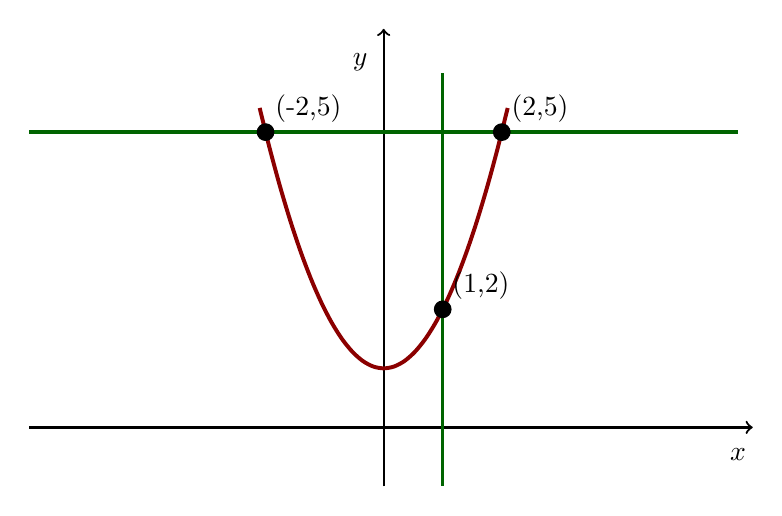
\begin{tikzpicture}[scale=0.75]
            \draw[thick, ->] (-6, 0) -- (6.25, 0);
            \draw[thick, ->] (0, -1) -- (0, 6.75);
            \node[overlay, below] at (6, -0.2) {$x$};
            \node[overlay, below] at (-0.4, 6.5) {$y$};   
            \draw[very thick,DarkGreen, -] (1, 6) -- (1, -1);        
            \draw[very thick,DarkGreen, -] (-6, 5) -- (6, 5);   
            \draw[DarkRed, line width = 0.50mm]   plot[smooth,domain=-2.1:2.1] (\x, {\x*\x+1});
            \filldraw[black] (2,5) circle (4pt) node[anchor=south west]{(2,5)};
            \filldraw[black] (-2,5) circle (4pt) node[anchor=south west]{(-2,5)};
            \filldraw[black] (1,2) circle (4pt) node[anchor=south west]{(1,2)};
            \end{tikzpicture}
            \end{center}               
        } 
        \else 
        \begin{center}
        \begin{tikzpicture}[scale=0.55]
        \draw[very thick, ->] (-6, 0) -- (6.25, 0);
        \draw[very thick, ->] (0, -6) -- (0, 6.25);
        \node[overlay, below] at (6, -0.2) {$x$};
        \node[overlay, below] at (-0.6, 6) {$y$};        
        \end{tikzpicture}
        \end{center}    
    \fi
    \end{parts}
\fi 




\ifnum \Version=3
    \question[6] Consider the non-linear system below.  
    \begin{align*}
        \dxdt &= (x-1)(y-2) , \qquad \dydt = y^2-x
    \end{align*}
    \begin{parts}
        \part Determine the locations of the critical points. 
        \ifnum \Solutions=1 {\color{DarkBlue} \\[12pt] 
        For a point to be a critical point, we need $x' = y' = 0$. If $x'$ is zero, then either $x=1$ or $y=2$. 
        \begin{itemize}
            \item When $x=1$, for $y'=0$ we need 
            \begin{align}
                y'&=0 = y^2 - x \quad \Rightarrow \quad y = \pm 1
            \end{align}
            There are critical points at $(1,\pm 1)$. 
            \item When $y=2$, for $y'=0$ we need 
            \begin{align}
                y'&=0 = y^2 - x  \quad \Rightarrow \quad x = 4 
            \end{align}
            There is a critical point at $(4, 2)$.             
        \end{itemize}
            } 
        \else 
        \vfill
        \fi
        \part Sketch the nullclines of the system on the axes below. Clearly indicate the critical points that you found in part (a). 
        \ifnum \Solutions=1 {\color{DarkBlue} \\[12pt] 
        The curves are shown below. The green lines are the x nullclines, and the red curve is the y nullcline. There are exactly three critical points. 
            \begin{center}
            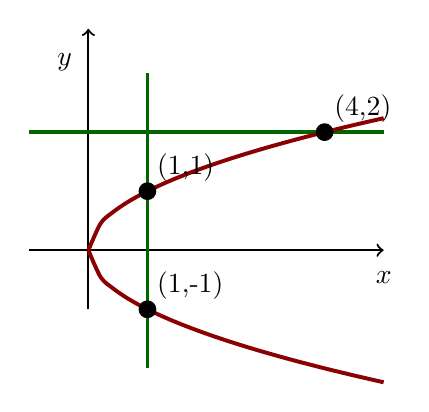
\begin{tikzpicture}[scale=0.75]
            \draw[thick, ->] (-1, 0) -- (5, 0);
            \draw[thick, ->] (0, -1) -- (0, 3.75);
            \node[overlay, below] at (5, -0.2) {$x$};
            \node[overlay, below] at (-0.4, 3.5) {$y$};   
            \draw[very thick,DarkGreen, -] (1, 3) -- (1, -2);        
            \draw[very thick,DarkGreen, -] (-1, 2) -- (5, 2);   
            \draw[DarkRed, line width = 0.50mm]   plot[smooth,domain=0:5] (\x, {\x^(1/2))} );
            \draw[DarkRed, line width = 0.50mm]   plot[smooth,domain=0:5] (\x, {-\x^(1/2))} );
            \filldraw[black] (4,2) circle (4pt) node[anchor=south west]{(4,2)};
            \filldraw[black] (1,1) circle (4pt) node[anchor=south west]{(1,1)};
            \filldraw[black] (1,-1) circle (4pt) node[anchor=south west]{(1,-1)};
            \end{tikzpicture}
            \end{center}               
        } 
        \else 
        \begin{center}
        \begin{tikzpicture}[scale=0.55]
        \draw[very thick, ->] (-6, 0) -- (6.25, 0);
        \draw[very thick, ->] (0, -6) -- (0, 6.25);
        \node[overlay, below] at (6, -0.2) {$x$};
        \node[overlay, below] at (-0.6, 6) {$y$};        
        \end{tikzpicture}
        \end{center}    
    \fi
    \end{parts}
\fi 


\ifnum \Version=6
    \question[4] Consider the non-linear system below.  
    \begin{align*}
        \dxdt &= (x-2)(y-1) , \qquad \dydt = 2y^2-x
    \end{align*}
    \begin{parts}
        \part Determine the locations of the critical points. 
        \ifnum \Solutions=1 {\color{DarkBlue} \\[12pt] 
        For a point to be a critical point, we need $x' = y' = 0$. If $x'$ is zero, then either $x=2$ or $y=1$. 
        \begin{itemize}
            \item When $x=2$, for $y'=0$ we need 
            \begin{align}
                y'&=0 = 2y^2 - x \quad \Rightarrow \quad y = \pm 1
            \end{align}
            There are critical points at $(2,\pm 1)$. 
            \item When $y=1$, for $y'=0$ we need 
            \begin{align}
                y'&=0 = 2y^2 - x  \quad \Rightarrow \quad x = 2
            \end{align}
            There is a critical point at $(2,1)$, which we already had.          
        \end{itemize}
            } 
        \else 
        \vfill
        \fi
        \part Sketch the nullclines of the system on the axes below. Clearly indicate the critical points that you found in part (a). 
        \ifnum \Solutions=1 {\color{DarkBlue} \\[12pt] 
        The curves are shown below. The green lines are the x nullclines, and the red curve is the y nullcline. There are exactly three critical points. 
            \begin{center}
            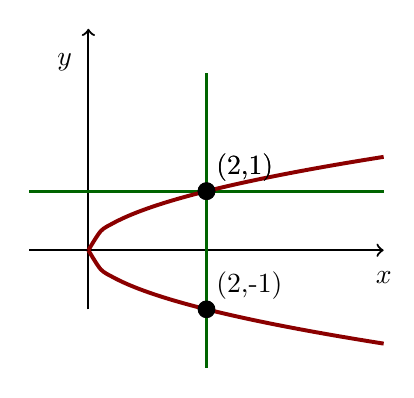
\begin{tikzpicture}[scale=0.75]
            \draw[thick, ->] (-1, 0) -- (5, 0);
            \draw[thick, ->] (0, -1) -- (0, 3.75);
            \node[overlay, below] at (5, -0.2) {$x$};
            \node[overlay, below] at (-0.4, 3.5) {$y$};   
            \draw[very thick,DarkGreen, -] (2, 3) -- (2, -2);        
            \draw[very thick,DarkGreen, -] (-1, 1) -- (5, 1);   
            \draw[DarkRed, line width = 0.50mm]   plot[smooth,domain=0:5] (\x, {(\x/2)^(1/2))} );
            \draw[DarkRed, line width = 0.50mm]   plot[smooth,domain=0:5] (\x, {-(\x/2)^(1/2))} );
            \filldraw[black] (2,1) circle (4pt) node[anchor=south west]{(2,1)};
            \filldraw[black] (2,1) circle (4pt) node[anchor=south west]{(2,1)};
            \filldraw[black] (2,-1) circle (4pt) node[anchor=south west]{(2,-1)};
            \end{tikzpicture}
            \end{center}               
        } 
        \else 
        \begin{center}
        \begin{tikzpicture}[scale=0.55]
        \draw[very thick, ->] (-6, 0) -- (6.25, 0);
        \draw[very thick, ->] (0, -6) -- (0, 6.25);
        \node[overlay, below] at (6, -0.2) {$x$};
        \node[overlay, below] at (-0.6, 6) {$y$};        
        \end{tikzpicture}
        \end{center}    
    \fi
    \end{parts}
\fi 


\ifnum \Version=7
    \question[4] Consider the non-linear system below.  
    \begin{align*}
        \dxdt &= (x-1)(y-5) , \qquad \dydt = y-x^2-1
    \end{align*}
    \begin{parts}
        \part Determine the locations of the critical points. 
        \ifnum \Solutions=1 {\color{DarkBlue} \\[12pt] 
        For a point to be a critical point, we need $x' = y' = 0$. If $x'$ is zero, then either $x=1$ or $y=5$. 
        \begin{itemize}
            \item When $x=1$, for $y'=0$ we need 
            \begin{align}
                y'&=0 = y - x^2 - 1 \quad \Rightarrow \quad y = 1^2+1 = 2
            \end{align}
            There is a critical point at $(1,2)$. 
            \item When $y=5$, for $y'=0$ we need 
            \begin{align}
                y'&=0 = y - x^2 - 1 \quad \Rightarrow \quad x^2 = 5 - 1 \quad \Rightarrow \quad x = \pm 2
            \end{align}
            There are critical points at $(\pm 2, 5)$.             
        \end{itemize}
            } 
        \else 
        \vfill
        \fi
        \part Sketch the nullclines of the system on the axes below. Clearly indicate the critical points that you found in part (a). 
        \ifnum \Solutions=1 {\color{DarkBlue} \\[12pt] 
        The curves are shown below. The green lines are the x nullclines, and the red curve is the y nullcline. There are exactly three critical points. 
            \begin{center}
            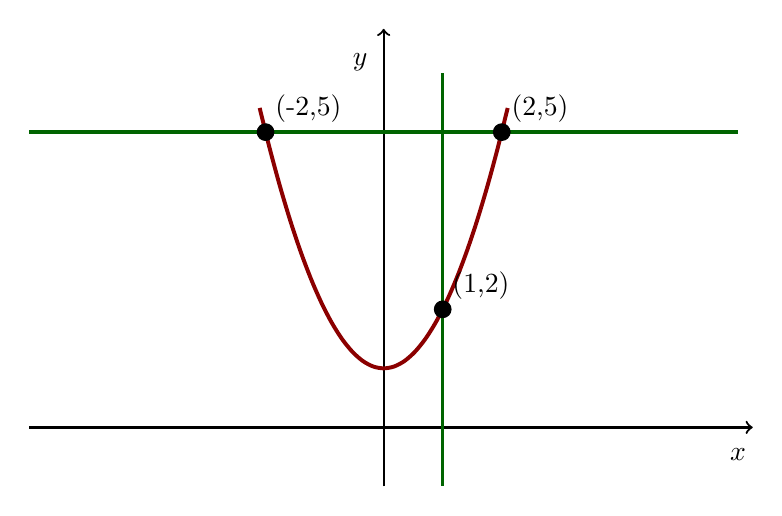
\begin{tikzpicture}[scale=0.75]
            \draw[thick, ->] (-6, 0) -- (6.25, 0);
            \draw[thick, ->] (0, -1) -- (0, 6.75);
            \node[overlay, below] at (6, -0.2) {$x$};
            \node[overlay, below] at (-0.4, 6.5) {$y$};   
            \draw[very thick,DarkGreen, -] (1, 6) -- (1, -1);        
            \draw[very thick,DarkGreen, -] (-6, 5) -- (6, 5);   
            \draw[DarkRed, line width = 0.50mm]   plot[smooth,domain=-2.1:2.1] (\x, {\x*\x+1});
            \filldraw[black] (2,5) circle (4pt) node[anchor=south west]{(2,5)};
            \filldraw[black] (-2,5) circle (4pt) node[anchor=south west]{(-2,5)};
            \filldraw[black] (1,2) circle (4pt) node[anchor=south west]{(1,2)};
            \end{tikzpicture}
            \end{center}               
        } 
        \else 
        \begin{center}
        \begin{tikzpicture}[scale=0.55]
        \draw[very thick, ->] (-6, 0) -- (6.25, 0);
        \draw[very thick, ->] (0, -6) -- (0, 6.25);
        \node[overlay, below] at (6, -0.2) {$x$};
        \node[overlay, below] at (-0.6, 6) {$y$};        
        \end{tikzpicture}
        \end{center}    
    \fi
    \end{parts}
\fi 

        \ifnum \Solutions=0
\newpage 
\fi
\ifnum \Version=1
\question[5] Consider the non-linear system below.  
\begin{align*}
    \dxdt &= x^2+y-2x-12 , \qquad \dydt = y-x-6
\end{align*}
The critical points are located at $(-2,4)$ and $(3,9)$. 
\begin{parts}
    \part Compute the Jacobian matrix, $J$, for the approximating linear system. 
    \ifnum \Solutions=1 {\color{DarkBlue}
        \begin{align}
            F &= x'\\
            G &= y' \\
            J &= \begin{pmatrix} F_x&F_y\\ G_x & G_y\end{pmatrix} = \begin{pmatrix} 2x-2&1\\-1&1\end{pmatrix}
        \end{align}
        } 
    \else 
    \vfill
    \fi        
    \part Use eigenvalues to classify the critical point at $(-2,4)$ according to stability (stable, unstable, asymptotically stable) and type (saddle, proper node, etc).
    \ifnum \Solutions=1 {\color{DarkBlue} \\[12pt] 
        At $(-2,4)$, $J = \begin{pmatrix} -6&1\\-1&1\end{pmatrix}$. The eigenvalues are the roots of \begin{align}
            (-6-\lambda)(1-\lambda)+1 = \lambda^2 +5\lambda - 5
        \end{align}
        Thus 
        \begin{align}
            \lambda = -\frac52 \pm \frac12 \sqrt{25-4\cdot(-5)} = -\frac52 \pm \frac{\sqrt{45}}{2}
        \end{align}
        $\lambda \in \mathbb R$, and the eigenvalues have opposite signs. The critical point is an unstable saddle. 
        } 
    \else 
    \vfill
    \fi
    \part Use eigenvalues to classify the critical point at $(3,9)$ according to stability (stable, unstable, asymptotically stable) and type (saddle, proper node, etc).
    \ifnum \Solutions=1 {\color{DarkBlue} \\[12pt] 
        At $(3,9)$, $J = \begin{pmatrix} 4&1\\-1&1\end{pmatrix}$. The eigenvalues are the roots of \begin{align}
            (4-\lambda)(1-\lambda)+1 = \lambda^2 - 5\lambda +5 
        \end{align}
        Thus 
        \begin{align}
            \lambda = \frac52 \pm \frac12 \sqrt{25-4\cdot(5)} = \frac52 \pm \frac{\sqrt{5}}{2}
        \end{align}
        $\lambda \in \mathbb R$, and the eigenvalues both positive. The critical point is an unstable node. 
    } 
    \else 
    \vfill
\fi
\end{parts}
\fi



\ifnum \Version=2
\question[6] Consider the non-linear system below.  
\begin{align*}
    \dxdt &= x(1-x-y) , \qquad \dydt = y(2-x-y)
\end{align*}
The critical points are located at $(0,0)$, $(0,2)$, and $(1,0)$. 
\begin{parts}
    \part Compute the Jacobian matrix, $J$, for the approximating linear system. 
    \ifnum \Solutions=1 {\color{DarkBlue} \\
    Set $ F = x'$ and $G = y'$. Then
        \begin{align}
            F_x &= 1 - 2x -y\\
            F_y &= -x \\
            G_x &= 2-x-2y \\
            G_y &= -y \\
            J &= \begin{pmatrix} F_x&F_y\\ G_x & G_y\end{pmatrix} = \begin{pmatrix} -1-x-2y & -x\\-y&2-x-2y \end{pmatrix}
        \end{align}
        } 
    \else 
    \vfill
    \fi        
    \part Use eigenvalues to classify the critical point at $(0,0)$ according to stability (stable, unstable, asymptotically stable) and type (saddle, proper node, etc).
    \ifnum \Solutions=1 {\color{DarkBlue} \\[12pt] 
        At $(0,0)$, $J = \begin{pmatrix} 1&0\\0&2\end{pmatrix}$. The eigenvalues are $\lambda = 1,2$. \\ Thus the critical point is an \textbf{unstable node}. 
        } 
    \else 
    \vfill
    \fi
    \part Use eigenvalues to classify the critical point at $(0,2)$ according to stability (stable, unstable, asymptotically stable) and type (saddle, proper node, etc).
    \ifnum \Solutions=1 {\color{DarkBlue} \\[12pt] 
        At $(0,2)$, $J = \begin{pmatrix} -1&0\\-2&-4\end{pmatrix}$. The eigenvalues are $\lambda = -1,-4$. \\Thus the critical point is a \textbf{stable node}. 
        } 
    \else 
    \vfill
    \fi
    \part Use eigenvalues to classify the critical point at $(1,0)$ according to stability (stable, unstable, asymptotically stable) and type (saddle, proper node, etc).
    \ifnum \Solutions=1 {\color{DarkBlue} \\[12pt] 
        At $(1,0)$, $J = \begin{pmatrix} -1&-1\\0&1\end{pmatrix}$. The eigenvalues are $\lambda = \pm 1$. \\ Thus the critical point is an \textbf{unstable saddle}. 
        } 
    \else 
    \vfill
    \fi    
\end{parts}
\fi










\ifnum \Version>5
\question[6] Consider the non-linear system below.  
\begin{align*}
    \dxdt &= x(4-x-y) , \qquad \dydt = y(6-2x-y)
\end{align*}
\begin{parts}
    \part Compute the Jacobian matrix, $J$, for the approximating linear system. 
    \ifnum \Solutions=1 {\color{DarkBlue} \\
    Set $ F = x'$ and $G = y'$. Then
        \begin{align}
            F &= 4x - x^2 - xy \\
            G &= 6y -2xy - y^2 \\
            J &= \begin{pmatrix} F_x&F_y\\ G_x & G_y\end{pmatrix} 
            = \begin{pmatrix} 4-2x-y & -x\\-2y& 6-2x-2y \end{pmatrix}
        \end{align}
        } 
    \else 
    \vfill
    \fi        
    \part Use eigenvalues to classify the critical point at $(0,6)$ according to stability (stable, unstable, asymptotically stable) and type (saddle, proper node, etc).
    \ifnum \Solutions=1 {\color{DarkBlue} \\[12pt] 
        At $(0,0)$, $J = \begin{pmatrix} -2&0\\-12&-6\end{pmatrix}$. The eigenvalues are $\lambda = -2, -6$. The CP is a \textbf{stable node}. 
        } 
    \else 
    \vfill
    \fi
    \part Use eigenvalues to classify the critical point at $(2,2)$ according to stability (stable, unstable, asymptotically stable) and type (saddle, proper node, etc).
    \ifnum \Solutions=1 {\color{DarkBlue} \\[12pt] 
        At $(0,2)$, $J = \begin{pmatrix} -2&-2\\-4&-2\end{pmatrix}$. Eigenvalues:
        \begin{align}
            0 &= (\lambda + 2)^2 - 8 = \lambda^2 + 4\lambda -4  \\
            \lambda &= -2 \pm \frac12 \sqrt{16 + 16} = -2 \pm 2\sqrt 2
        \end{align}\\Thus the critical point is an \textbf{unstable saddle}. 
        } 
    \else 
    \vfill
    \fi
\end{parts}
\fi

  
        \ifnum \Solutions=0
\newpage 
\fi

\ifnum \Version=1    
\question[2] 
Compute the Laplace transform of the function below. Do not leave your answer in terms of an integral. Please show your work. 
$$y(t) = \begin{cases} 0, \quad 0 \le t < 1 \\ t-2, \quad 1 \le t < 3 \\ 0, \quad 3 \le t < \infty\end{cases}$$
\ifnum \Solutions=1 {\color{DarkBlue} \\[12pt] 
There are a few different ways to solve this. Any of the approaches below are sufficient. 
\subsection*{Method 1: Direct Integration }
Direct integration requires integration by parts, but using the definition of the Laplace Transform:
    \begin{align}
        \int_0^{\infty} e^{-st} y(t) \, dt 
        &= \int_1^{3} e^{-st} \, (t-2) \, dt \\
        &= \int_1^{3} te^{-st}  \, dt - 2 \int_1^{3} e^{-st}  \, dt \\
        &=  \left. t\cdot \frac{-1}{s}e^{-st} \right|_1^3
        - \int_1^{3} \frac{-1}{s}e^{-st} \, dt 
        -2 \left( \left. \frac{-1}{s}e^{-st}\right|_{t=1}^{t=3}\right) \\
        &=  \frac{-1}{s}\left( 3e^{-3s} - e^{-s} \right)  
        + \frac{1}{s} \int_1^{3} e^{-st} \, dt 
        + \frac{2}{s} \left(  e^{-3s} - e^{-s} \right) \\
        &=  \frac{-1}{s}\left( 3e^{-3s} - e^{-s} \right)  
        + \frac{1}{s} \left( \left. \frac{-1}{s}e^{-st}\right|_{t=1}^{t=3}\right) \, dt 
        + \frac{2}{s} \left(  e^{-3s} - e^{-s} \right) \\     
        &=  \frac{-1}{s}\left( 3e^{-3s} - e^{-s} \right)  
        - \frac{1}{s^2} \left(  e^{-3s} - e^{-s} \right) 
        + \frac{2}{s} \left(  e^{-3s} - e^{-s} \right) \\      
        &= - \frac{1}{s^2} \left(  e^{-3s} - e^{-s} \right) 
        - \frac{ e^{-3s}}{s}   - \frac{e^{-s}}{s}  \\   
        &= \frac{e^{-s}}{s^2} - \frac{e^{-3s}}{s^2} 
        - \frac{ e^{-3s}}{s}   - \frac{e^{-s}}{s}           
    \end{align}
    \subsection*{Method 2: Step Functions}
    We could also use the table of transforms, specifically the transform of the step function $u_c(t)$ and its product with another function. 
    \begin{align}
        y(t) &= 0u_{0,1} + (t-2)u_{1,3} + 0u_{3} 
        =(t-2)(u_1-u_3) 
        = tu_1-tu_3 - 2u_1 + 2 u_3 
    \end{align}   
    At this point we can either take the transform and use the derivative theorem (in the table) to work out the transform of $tu_1$ and $tu_3$, or we can use the following trick:
    \begin{align}
        y(t) &= tu_1-tu_3 - 2u_1 + 2 u_3 \\
        &= (t+1-1)u_1-(t+3-3)u_3 - 2u_1 + 2 u_3 \\
        &= (t-1)u_1 + u_1 -(t-3)u_3 - 3u_3 - 2u_1 + 2 u_3 \\
        &= (t-1)u_1 -(t-3)u_3 - u_1 - u_3 
    \end{align}
    Using the table of transforms the Laplace transform is
    \begin{align}
        Y(s) = \frac{e^{-s}}{s^2} - \frac{e^{-3s}}{s^2} - \frac{e^{-s}}{s} - \frac{e^{-3s}}{s}
    \end{align}
} 
\else 
    \vfill
    \begin{center}
        \textit{This remainder of this page can be used for scratch work. }
    \end{center}
    \vfill
\fi
\fi


\ifnum \Version=5
\question[2] 
Compute the Laplace transform of the function below. Do not leave your answer in terms of an integral. Please show your work. 
$$y(t) = \begin{cases} 0, \quad 0 \le t < 1 \\ 4, \quad 1 \le t < 3 \\ 0, \quad 3 \le t < \infty\end{cases}$$
\ifnum \Solutions=1 {\color{DarkBlue} \\[12pt] 
There are a few different ways to solve this. Any of the approaches below are sufficient. 
\subsection*{Method 1: Direct Integration }
Direct integration uses the definition of the Laplace Transform:
    \begin{align}
        \int_0^{\infty} e^{-st} y(t) \, dt 
        = \int_1^{3} e^{-st} \, 4 \, dt 
        &= 4\int_1^{3} e^{-st}  \, dt  \\         
        &= 4\left.\frac{-1}{s} e^{-st} \right|_1^3  \\         
        &= \frac{-4}{s} \left(e^{-3s}  - e^{-s} \right)     
    \end{align}
    \subsection*{Method 2: Step Functions}
    We could also use the table of transforms, specifically the transform of the step function $u_c(t)$ and its product with another function. 
    \begin{align}
        y(t) &= 0u_{0,1} + 4u_{1,3} + 0u_{3} 
        =4(u_1-u_3) 
        = 4u_1 - 4 u_3 
    \end{align}   
    Using the table of transforms the Laplace transform is
    \begin{align}
        Y(s) = 4 \frac{e^{-s}}{s} - 4\frac{e^{-3s}}{s}
    \end{align}
    \newpage
} 
\else 
    \vfill
    \begin{center}
        \textit{This remainder of this page can be used for scratch work. }
    \end{center}
    \vfill
\fi
\fi







\ifnum \Version=6
\question[3] 
The function $f(t)$ is periodic, has period $4$, and 
        $$f(t) = \begin{cases} e^{-3t}, \quad 0 \le t < 2 \\ 0, \quad 2 \le t < 4 \end{cases}$$
        Compute the Laplace transform of $f(t)$. Do not leave your answer in terms of an integral. Please show your work. 

\ifnum \Solutions=1 {\color{DarkBlue} 
    We use the formula for a periodic function with $T=4$. 
    
        With $T=4$,
        
        \begin{align}
            \mathcal{L}\{f(t)\} &=  \frac{\int_{0}^{T} e^{-st} f(t) dt}{1 - e^{-Ts}} \\
            &= \frac{1}{1 - e^{-4s}} \left( \int_{0}^{2} e^{-st} e^{-3t} dt + \int_2^4 0 \, dt \right)\\
            &= \frac{1}{1 - e^{-4s}} \cdot \frac{1}{-s-3} \left. e^{(-s-3)t}\right|_0^2 \\
            &= -\frac{1}{1 - e^{-4s}} \cdot \frac{1}{s+3} \left( e^{-2(s+3)} - 1 \right)
        \end{align}
        \newpage
} 
\else 
    \newpage
    \begin{center}
        \textit{This remainder of this page can be used for scratch work. }
    \end{center}
    \vfill
\fi
\fi



\ifnum \Version=7
\question[3] 
The function $f(t)$ is periodic, has period $4$, and 
        $$f(t) = \begin{cases} e^{-2t}, \quad 0 \le t < 3 \\ 0, \quad 3 \le t < 4 \end{cases}$$
        Compute the Laplace transform of $f(t)$. Do not leave your answer in terms of an integral. Please show your work. 

\ifnum \Solutions=1 {\color{DarkBlue} 
    We use the formula for a periodic function with $T=4$. 
    
        With $T=4$,
        
        \begin{align}
            \mathcal{L}\{f(t)\} &=  \frac{\int_{0}^{T} e^{-st} f(t) dt}{1 - e^{-Ts}} \\
            &= \frac{1}{1 - e^{-4s}} \left( \int_{0}^{3} e^{-st} e^{-2t} dt + \int_3^4 0 \, dt \right)\\
            &= \frac{1}{1 - e^{-4s}} \cdot \frac{1}{-s-2} \left. e^{(-s-2)t}\right|_0^3 \\
            &= -\frac{1}{1 - e^{-4s}} \cdot \frac{1}{s+2} \left( e^{-3(s+2)} - 1 \right)
        \end{align}
} 
\else 
    \newpage
    \begin{center}
        \textit{This remainder of this page can be used for scratch work. }
    \end{center}
    \vfill
\fi
\fi




    \fi 
\end{questions}